%%%%%%%%%%%%%%%%%%%%%%%%%%%%%%%%%%%%%%%%%%%%%%%%%%%
%% LaTeX book template                           %%
%% Author:  Amber Jain (http://amberj.devio.us/) %%
%% License: ISC license                          %%
%%%%%%%%%%%%%%%%%%%%%%%%%%%%%%%%%%%%%%%%%%%%%%%%%%%

\documentclass[a4paper,11pt,oneside]{book}
\usepackage{modulestyle}

%%%%%%%%%%%%%%%%%%%%%%%%%%%%%%%%%%%%%%%%%%%%%%%%%%%%%%%%%
% Source: http://en.wikibooks.org/wiki/LaTeX/Hyperlinks %
%%%%%%%%%%%%%%%%%%%%%%%%%%%%%%%%%%%%%%%%%%%%%%%%%%%%%%%%%

%%%%%%%%%%%%%%%%%%%%%%%%%%%%%%%%%%%%%%%%%%%%%%%%%%%%%%%%%%%%%%%%%%%%%%%%%%%%%%%%
% 'dedication' environment: To add a dedication paragraph at the start of book %
% Source: http://www.tug.org/pipermail/texhax/2010-June/015184.html            %
%%%%%%%%%%%%%%%%%%%%%%%%%%%%%%%%%%%%%%%%%%%%%%%%%%%%%%%%%%%%%%%%%%%%%%%%%%%%%%%%
\newenvironment{dedication}
{
   \cleardoublepage
   \thispagestyle{empty}
   \vspace*{\stretch{1}}
   \hfill\begin{minipage}[t]{0.66\textwidth}
   \raggedright
}
{
   \end{minipage}
   \vspace*{\stretch{3}}
   \clearpage
}

%%%%%%%%%%%%%%%%%%%%%%%%%%%%%%%%%%%%%%%%%%%%%%%%
% Chapter quote at the start of chapter        %
% Source: http://tex.stackexchange.com/a/53380 %
%%%%%%%%%%%%%%%%%%%%%%%%%%%%%%%%%%%%%%%%%%%%%%%%
\makeatletter
\renewcommand{\@chapapp}{}% Not necessary...
\newenvironment{chapquote}[2][2em]
  {\setlength{\@tempdima}{#1}%
   \def\chapquote@author{#2}%
   \parshape 1 \@tempdima \dimexpr\textwidth-2\@tempdima\relax%
   \itshape}
  {\par\normalfont\hfill--\ \chapquote@author\hspace*{\@tempdima}\par\bigskip}
\makeatother

%%%%%%%%%%%%%%%%%%%%%%%%%%%%%%%%%%%%%%%%%%%%%%%%%%%
% First page of book which contains 'stuff' like: %
%  - Book title, subtitle                         %
%  - Book author name                             %
%%%%%%%%%%%%%%%%%%%%%%%%%%%%%%%%%%%%%%%%%%%%%%%%%%%

\newcommand{\BookTitle}{Data Structures and Algorithms}
\newcommand{\BookTitleFootnote}{A course in the Bachelor of Science in Computer
Science/Information Technology/Information Systems program.}

\newcommand{\BookSubtitle}{A Study Guide for Students of Sorsogon State University - Bulan Campus}
\newcommand{\BookSubtitleFootnote}{This book is a study guide for students of
Sorsogon State University - Bulan Campus taking up the course Data Structures
and Algorithms.}

\newcommand{\BookAuthorFirstName}{Jarrian Vince}
\newcommand{\BookAuthorLastName}{Gojar}
\newcommand{\BookAuthorName}{Jarrian Vince G. Gojar}
\newcommand{\BookAuthorURL}{https://github.com/godkingjay}

% Book's title and subtitle
\title{\Huge \textbf{\BookTitle}  \footnote{\BookTitleFootnote} \\
\huge \BookSubtitle \footnote{\BookSubtitleFootnote}}

% Author
\author{\textsc{\BookAuthorName}\thanks{\url{\BookAuthorURL}}}

\begin{document}

\frontmatter
\maketitle

%%%%%%%%%%%%%%%%%%%%%%%%%%%%%%%%%%%%%%%%%%%%%%%%%%%%%%%%%%%%%%%
% Add a dedication paragraph to dedicate your book to someone %
%%%%%%%%%%%%%%%%%%%%%%%%%%%%%%%%%%%%%%%%%%%%%%%%%%%%%%%%%%%%%%%
\begin{dedication}
Sorsogon State University - Bulan Campus
\end{dedication}

%%%%%%%%%%%%%%%%%%%%%%%%%%%%%%%%%%%%%%%%%%%%%%%%%%%%%%%%%%%%%%%%%%%%%%%%
% Auto-generated table of contents, list of figures and list of tables %
%%%%%%%%%%%%%%%%%%%%%%%%%%%%%%%%%%%%%%%%%%%%%%%%%%%%%%%%%%%%%%%%%%%%%%%%
\tableofcontents
\listoffigures
\listoftables
\lstlistoflistings

\mainmatter

%%%%%%%%%%%
% Preface %
%%%%%%%%%%%
\chapter*{Preface}
% A Quote all about Data Structures and Algorithms
\begin{chapquote}{Linus Torvalds}
``Bad programmers worry about the code. Good programmers worry about data structures and their relationships.''
\end{chapquote}

\noindent \BookAuthorName \\
\noindent \url{\BookAuthorURL}

%%%%%%%%%%%%%%%%%%%%%%%%%%%%%%%%%%%%
%%%%%~ NEW CHAPTER STARTS HERE %%%%%
%%%%%%%%%%%%%%%%%%%%%%%%%%%%%%%%%%%%
\chapter{Introduction to Data Structures and Algorithms}

\section{Introduction}

Data structures and algorithms are one of the fundamental components of computer
science. They are essential for solving complex problems efficiently and
effectively. Data structures are used to store and organize data in a computer
so that it can be accessed and manipulated efficiently. Algorithms
are step-by-step procedures or formulas for solving a problem. They are the
instructions that tell a computer how to perform a task.

In this course, we will learn about the fundamental data structures and
algorithms that are used in computers. We will study how to design,
implement, and analyze data structures and algorithms to solve real-world
problems. By the end of this course, you will have a solid foundation in
data structures and algorithms that will help you become a better programmer
and problem solver.

\section{Setup and Installation}

In this course, we will be using the C++ programming language to implement
data structures and algorithms. C++ is a powerful and versatile programming
language that is widely used in the field of computer science. To get started,
you will need to install a C++ compiler and an integrated development
environment (IDE) on your computer.

\subsection{C++ Compiler Installation}

The first step is to install a C++ compiler on your computer. A compiler is
a program that translates source code written in a programming language into
machine code that can be executed by a computer. There are several C++
compilers available, but we recommend using the GNU Compiler Collection (GCC)
which is a free and open-source compiler that supports multiple programming
languages including C++.

\subsubsection{Windows}

To install GCC on Windows, you can use the MinGW (Minimalist GNU for Windows)
project which provides a port of GCC to Windows. You can download the MinGW
installer from the MinGW website and follow the installation instructions.
You can install MinGW by following the instructions here:
\url{https://code.visualstudio.com/docs/languages/cpp#_example-install-mingwx64-on-windows}

\subsection{Visual Studio Code Installation}

The next step is to install an integrated development environment (IDE) on
your computer. An IDE is a software application that provides comprehensive
facilities to computer programmers for software development. We recommend
using Visual Studio Code which is a free and open-source IDE developed by
Microsoft. You can download Visual Studio Code from the official website
and follow the installation instructions: \url{https://code.visualstudio.com/Download}

Other than Visual Studio Code, you also need to install the C/C++ extension
for Visual Studio Code. You can install the C/C++ extension by following the
instructions here: \url{https://code.visualstudio.com/docs/languages/cpp}

\subsection{Testing the Installation}

To test if the installation was successful, you can create a simple C++
program and compile it using the C++ compiler. Open Visual Studio Code and
create a new file with the following C++ code:

\begin{lstlisting}[language=C++, caption={Hello World Program}]
#include <iostream>
namespace std;

int main() {
    cout << "Hello, World!" << endl;
    return 0;
}
\end{lstlisting}

Save the file with a .cpp extension (e.g., hello.cpp) and open a terminal
window in Visual Studio Code. Compile the program using the following command:

\begin{lstlisting}[language=bash, caption={Compiling the Program}]
g++ hello.cpp -o hello
\end{lstlisting}

If there are no errors, you can run the program by executing the following
command:

\begin{lstlisting}[language=bash, caption={Running the Program}]
./hello
\end{lstlisting}

If everything is set up correctly, you should see the output "Hello, World!"
printed on the screen.

\section{What are Data Structures?}

A \textbf{\textit{data structure}} is a way of organizing and storing data in a computer so
that it can be accessed and manipulated efficiently. Data structures provide a
way to manage large amounts of data effectively for various applications. They
define the relationship between the data, and the operations that can be
performed on the data. There are many different types of data structures that
are used in computer science, each with its own strengths and weaknesses. The use
of the right data structure can significantly improve the performance of an
algorithm and make it more efficient.

\section{What are Algorithms?}

An \textbf{\textit{algorithm}} is a step-by-step procedure or formula for solving a problem.
It is a sequence of well-defined instructions that take some input and produce
an output. Algorithms are used to solve complex problems and perform various
tasks efficiently. They are the instructions that tell a computer how to perform
a task. Algorithms are essential for writing computer programs and developing
software applications. The efficiency of an algorithm is measured by its time
complexity and space complexity.

\section{Why Study Data Structures and Algorithms?}

Data structures and algorithms are essential topics in computer science and
software engineering. They are one of the fundamental components of computer
science and are used in various applications such as operating systems,
database management systems, networking, artificial intelligence, and many
others. A good understanding of data structures and algorithms will help
you become a better programmer and problem solver. In addition, many companies
use data structures and algorithms as part of their technical interviews to
assess the problem-solving skills of candidates. Therefore, studying data
structures and algorithms is essential for anyone pursuing a career in
software engineering or software development.

\section{Basic Terminologies}

Before we dive into the details of data structures and algorithms, let's
understand some basic terminologies that might be helpful in understanding
the concepts better.

\subsection{Data}

\textbf{\textit{Data}} is a collection of facts, figures, or information that
can be used for analysis or reference. It can be in the form of numbers, text,
images, audio, video, or any other format. Data is the raw material that is
processed by a computer to produce meaningful information.

\subsection{Data Object}

A \textbf{\textit{data object}} is an instance of a data structure that contains
data along with the operations that can be performed on the data. It is an
abstraction of a real-world entity that is represented in a computer program.

\subsection{Data Type}

A \textbf{\textit{data type}} is a classification of data that tells the compiler
or interpreter how the programmer intends to use the data. It defines the
operations that can be performed on the data, the values that can be stored
in the data, and the memory space required to store the data.

\subsubsection{Primitive Data Types}

Primitive data types are the basic data types that are built into the programming
language. They are used to store simple values such as integers, floating-point
numbers, characters, and booleans. Examples of primitive data types include
int, float, char, and bool. The following are the common primitive data types
used in programming:

\paragraph{Integer (int)}

The \textbf{\textit{integer}} data type is used to store whole numbers without any decimal points.
It can be either signed or unsigned, depending on whether it can store negative
values or not. An integer's value can range from -2,147,483,648 to 2,147,483,647
and takes 4 bytes of memory.

\begin{lstlisting}[language=C++, caption={Integer Data Type}]
int x = 10;
\end{lstlisting}


\paragraph{Character (char)}

The \textbf{\textit{character}} data type is used to store a single character such as a letter,
digit, or special symbol. It is represented by a single byte of memory. A char
value can range from -128 to 127 or 0 to 255, depending on whether it is signed
or unsigned. These values are represented using ASCII codes.

\begin{lstlisting}[language=C++, caption={Character Data Type}]
char c = 'A';
\end{lstlisting}

\paragraph{Boolean (bool)}

The \textbf{\textit{boolean}} data type is used to store true or false values. It is represented
by a single byte of memory. A bool value can be either true or false.

\begin{lstlisting}[language=C++, caption={Boolean Data Type}]
bool flag = true;
\end{lstlisting}

\paragraph{Floating-Point (float)}

The \textbf{\textit{floating-point}} data type is used to store real numbers with decimal points.
It can represent both integer and fractional parts of a number. It can be either
single precision or double precision, depending on the number of bits used to
store the value. A float value can range from 1.2E-38 to 3.4E+38 and takes 4
bytes of memory.

\begin{lstlisting}[language=C++, caption={Floating-Point Data Type}]
float y = 3.14;
\end{lstlisting}

\paragraph{Double (double)}

The \textbf{\textit{double}} data type is used to store real numbers with double precision. It can
represent both integer and fractional parts of a number with higher precision
than the float data type. A double value can range from 2.3E-308 to 1.7E+308 and
takes 8 bytes of memory.

\begin{lstlisting}[language=C++, caption={Double Data Type}]
double z = 3.14159;
\end{lstlisting}

\subsubsection{Non-primitive Data Types}

Non-primitive data types are more complex data types that are derived from primitive
data types. They are used to store collections of values or objects. Examples of
non-primitive data types include arrays, strings, structures, classes, and pointers.

\paragraph{Array (int, float, char, etc.)}

An \textbf{\textit{array}} is a collection of elements of the same data type that are stored in
contiguous memory locations. It is used to store multiple values of the same
type under a single name. The elements of an array can be accessed using an
index value. In C++, arrays are zero-indexed, which means the first element is
at index 0. Arrays also have a fixed size that is specified at the time of
declaration. If you need a dynamic size array, you can use a vector in C++.

\begin{lstlisting}[language=C++, caption={Array Data Type}]
int arr[5] = {1, 2, 3, 4, 5};
\end{lstlisting}

\paragraph{String (char)}

A \textbf{\textit{string}} is a collection of characters that are stored
as a sequence of characters terminated by a null character
'\textbackslash0'. It is used to represent text in a computer program.
Strings are treated as arrays of characters in C++.

\begin{lstlisting}[language=C++, caption={String Data Type}]
char str[] = "Hello, World!";
\end{lstlisting}

\paragraph{Structure}

A \textbf{\textit{structure}} is a user-defined data type that is used to
store a collection of different data types under a single name. It is used
to represent a record that contains multiple fields or members. Each field
in a structure can have a different data type.

\begin{lstlisting}[language=C++, caption={Structure Data Type}]
struct Person {
    char name[50];
    int age;
    float height;
};
\end{lstlisting}

\paragraph{Class}

A \textbf{\textit{class}} is a user-defined data type that is used to define
objects that contain data members and member functions. It is used to
implement object-oriented programming concepts such as encapsulation,
inheritance, and polymorphism.

\begin{lstlisting}[language=C++, caption={Class Data Type}]
class Circle {
    private:
        float radius;
    public:
        float getArea() {
            return 3.14 * radius * radius;
        }
};
\end{lstlisting}

% \paragraph{Pointer}

% A \textbf{\textit{pointer}} is a special type of data type that stores the
% memory address of another data type. It is used to store the address of a
% variable or object in memory. Pointers are used to implement dynamic
% memory allocation and to pass parameters by reference.

% \begin{lstlisting}[language=C++, caption={Pointer Data Type}]
% int x = 10;
% int *ptr = &x;

% cout << *ptr; // Output: 10
% \end{lstlisting}

\paragraph{Vector}

A \textbf{\textit{vector}} is a dynamic array that can grow or shrink in size
dynamically. It is a part of the Standard Template Library (STL) in C++ and
provides a more flexible alternative to fixed-size arrays. Vectors are used
to store a collection of elements of the same data type.

\begin{lstlisting}[language=C++, caption={Vector Data Type}]
vector<int> vec = {1, 2, 3, 4, 5};
\end{lstlisting}

\paragraph{List}

A \textbf{\textit{list}} is a linear data structure that is used to store a
collection of elements in a sequential order. It is a part of the Standard
Template Library (STL) in C++ and provides operations to insert, delete, and
access elements in the list. Lists are used to implement linked lists in C++.

\begin{lstlisting}[language=C++, caption={List Data Type}]
list<int> lst = {1, 2, 3, 4, 5};
\end{lstlisting}

There are different types of lists in C++, such as singly linked list, doubly
linked list, circular linked list, and circular doubly linked list, that provide different operations and
performance characteristics.

\subparagraph{Singly Linked List}

A \textbf{\textit{singly linked list}} is a linear data structure that is used
to store a collection of elements in a sequential order. Each element in the
list is stored in a node that contains the data and a pointer to the next node
in the list.

\begin{lstlisting}[language=C++, caption={Singly Linked List Data Type}]
struct Node {
    int data;
    Node *next;
};
\end{lstlisting}

\subparagraph{Doubly Linked List}

A \textbf{\textit{doubly linked list}} is a linear data structure that is used
to store a collection of elements in a sequential order. Each element in the
list is stored in a node that contains the data, a pointer to the next node,
and a pointer to the previous node in the list.

\begin{lstlisting}[language=C++, caption={Doubly Linked List Data Type}]
struct Node {
    int data;
    Node *next;
    Node *prev;
};
\end{lstlisting}

\subparagraph{Circular Linked List}

A \textbf{\textit{circular linked list}} is a linear data structure that is used
to store a collection of elements in a circular order. Each element in the list
is stored in a node that contains the data and a pointer to the next node in
the list. The last node in the list points back to the first node, creating a
circular structure.

\begin{lstlisting}[language=C++, caption={Circular Linked List Data Type}]
struct Node {
    int data;
    Node *next;
};
\end{lstlisting}

\subparagraph{Circular Doubly Linked List}

A \textbf{\textit{circular doubly linked list}} is a linear data structure that
is used to store a collection of elements in a circular order. Each element in
the list is stored in a node that contains the data, a pointer to the next node,
and a pointer to the previous node in the list. The last node in the list points
back to the first node, creating a circular structure.

\begin{lstlisting}[language=C++, caption={Circular Doubly Linked List Data Type}]
struct Node {
    int data;
    Node *next;
    Node *prev;
};
\end{lstlisting}

\paragraph{Stack}

A \textbf{\textit{stack}} is a linear data structure that follows the Last In
First Out (LIFO) principle. It is used to store a collection of elements in a
sequential order. The main operations on a stack are push (to insert an element)
and pop (to remove an element).

\begin{lstlisting}[language=C++, caption={Stack Data Type}]
stack<int> stk;
stk.push(1);
stk.push(2);
stk.push(3);
stk.push(4);
stk.pop();
\end{lstlisting}

\paragraph{Queue}

A \textbf{\textit{queue}} is a linear data structure that follows the First In
First Out (FIFO) principle. It is used to store a collection of elements in a
sequential order. The main operations on a queue are enqueue (to insert an
element) and dequeue (to remove an element).

\begin{lstlisting}[language=C++, caption={Queue Data Type}]
queue<int> que;
que.push(1);
que.push(2);
que.push(3);
que.push(4);
que.pop();
\end{lstlisting}

There are different types of queues in C++, such as linear queue, circular
queue, priority queue, and double-ended queue (deque), that provide different
operations and performance characteristics.

\subparagraph{Circular Queue}

A \textbf{\textit{circular queue}} is a type of queue that uses a circular
structure to store elements. Unlike a linear queue, a circular queue does not
have a fixed front and rear end. Instead, the front and rear ends wrap around
the ends of the queue. This allows the queue to reuse the space freed up by
dequeued elements. In C++, there is no built-in circular queue data type, but
you can implement one using an array and a few pointers.

\subparagraph{Priority Queue}

A \textbf{\textit{priority queue}} is a type of queue that stores elements
based on their priority. The element with the highest priority is dequeued
first. Priority queues are typically implemented using heaps, which are a
type of binary tree data structure.

\begin{lstlisting}[language=C++, caption={Priority Queue Data Type}]
priority_queue<int> pq;
pq.push(1);
pq.push(4);
pq.push(2);
pq.push(3);
pq.pop();
\end{lstlisting}

\subparagraph{Double-Ended Queue (Deque)}

A \textbf{\textit{double-ended queue}} or \textbf{\textit{deque}} is a type of
queue that allows elements to be inserted and removed from both ends. It is
a generalization of both stacks and queues and provides more flexibility in
manipulating elements.

\begin{lstlisting}[language=C++, caption={Deque Data Type}]
deque<int> dq;
dq.push_front(1);
dq.push_back(2);
dq.push_front(3);
dq.push_back(4);
dq.pop_front();
\end{lstlisting}

\paragraph{Tree}

A \textbf{\textit{tree}} is a non-linear data structure that is used to store
a collection of elements in a hierarchical order. It consists of nodes that
are connected by edges. The topmost node in a tree is called the root node,
and the nodes below it are called child nodes. Trees are used to represent
hierarchical relationships between elements.

\begin{lstlisting}[language=C++, caption={Tree Data Type}]
struct Node {
    int data;
    Node *left;
    Node *right;
};
\end{lstlisting}

There are different types of trees in computer science, such as binary trees,
binary search trees, AVL trees, red-black trees, and many others, that provide
different operations and performance characteristics.

\paragraph{Graph}

A \textbf{\textit{graph}} is a non-linear data structure that is used to store
a collection of elements and the relationships between them. It consists of
nodes (vertices) that are connected by edges. Graphs are used to represent
networks, social relationships, maps, and many other real-world applications.

\begin{lstlisting}[language=C++, caption={Graph Data Type}]
struct Graph {
    int V;
    list<int> *adj;
};
\end{lstlisting}

There are different types of graphs in computer science, such as directed graphs,
undirected graphs, weighted graphs, and many others, each with its own set of
advantages and disadvantages.

Another important thing to note is that ``Every tree is a graph, but not every
graph is a tree.''

\paragraph{Hash Map or Hash Table}

A \textbf{\textit{Hash Map}} is a data structure that is used to store a
collection of key-value pairs. It uses a hash function to map keys to values
and stores them in an array. Hash maps provide fast access to elements and
are used to implement associative arrays, sets, and dictionaries.

There are two ways to implement a hash map in C++: the ordered map using the
map class or using the unordered\_map class.

\begin{lstlisting}[language=C++, caption={Ordered Map Data Type}]
map<string, int> mp;
mp["one"] = 1;
mp["two"] = 2;
mp["three"] = 3;
\end{lstlisting}

\begin{lstlisting}[language=C++, caption={Unordered Map Data Type}]
unordered_map<string, int> ump;
ump["one"] = 1;
ump["two"] = 2;
ump["three"] = 3;
\end{lstlisting}

\paragraph{Set}

A \textbf{\textit{set}} is a data structure that is used to store a collection
of unique elements. It is used to implement the mathematical set abstraction
and provides operations to insert, delete, and search for elements.

There are two ways to implement a set in C++: the ordered set using the set
class or using the unordered\_set class.

\begin{lstlisting}[language=C++, caption={Ordered Set Data Type}]
set<int> st;
st.insert(1);
st.insert(2);
st.insert(3);
\end{lstlisting}

\begin{lstlisting}[language=C++, caption={Unordered Set Data Type}]
unordered_set<int> ust;
ust.insert(1);
ust.insert(2);
ust.insert(3);
\end{lstlisting}

\subsection{Abstract Data Type}

An \textbf{\textit{abstract data type (ADT)}} is a mathematical model that
defines a set of data values and operations that can be performed on those
values. It is an abstraction of a data structure that specifies the operations
that can be performed on the data without specifying how they are implemented.
\textit{Abstraction} refers to the process of hiding the implementation
details of a data structure and exposing only the essential features. An ADT
is defined by its interface, which includes the data values and operations
that can be performed on those values.

\subsection{Pointers}

A \textbf{\textit{pointer}} is a special type of data type that stores the
memory address of another data type. An ``address'' is a unique number that
identifies a location in memory. The memory address of a variable is the
location in memory where the variable is stored. Pointers are used to store
the address of a variable or object in memory. Pointers are used to implement
dynamic memory allocation and to pass parameters by reference.

\begin{figure}[h]
    \centering
    \begin{tikzpicture}
        \node (x) [draw, rectangle] {x = 10};
        \node (ptr) [draw, rectangle, right=of x] {ptr = 0x7fffbf7f1bdc};
        \draw[->] (ptr) -- (x);
    \end{tikzpicture}
    \caption{Pointer Example}
    \label{fig:pointer-example}
\end{figure}

Figure \ref{fig:pointer-example} shows an example of a pointer in C++. The
variable \texttt{x} stores the value 10, and the pointer \texttt{ptr} stores
the memory address of the variable \texttt{x}. The memory address is represented
as a hexadecimal number \texttt{0x7fffbf7f1bdc}.

\begin{lstlisting}[language=C++, caption={Pointer Data Type}]
int main() {
    int x = 10;
    int *ptr = &x;

    cout << *ptr; // Output: 10

    return 0;
}
\end{lstlisting}

In the above example, the pointer \texttt{ptr} stores the memory address of
the variable \texttt{x}. The \texttt{*} operator is used to dereference the
pointer and access the value stored at the memory address.

An example of an address of a variable is \texttt{0x7fffbf7f1bdc}. When you
dereference the pointer, you get the value stored at that address.

\subsubsection{Declaring Pointers}

To declare a pointer, you need to specify the data type of the variable or
object it points to. You can declare a pointer using the following syntax:

\begin{lstlisting}[language=C++, caption={Declaring Pointers}]
int *ptr;
\end{lstlisting}

In the above example, the pointer \texttt{ptr} is declared to point to an
integer variable. You can also declare a pointer to a structure, class, or
any other data type.

\subsubsection{Initializing Pointers}

To initialize a pointer, you need to assign it the memory address of a variable
or object. You can initialize a pointer using the address-of operator \texttt{\&}.
You can also initialize a pointer to \texttt{NULL} or \texttt{nullptr} to indicate
that it does not point to any memory location.

\begin{lstlisting}[language=C++, caption={Initializing Pointers}]
int x = 10;
int *ptr = &x;
\end{lstlisting}

In the above example, the pointer \texttt{ptr} is initialized with the memory
address of the variable \texttt{x}.

\subsubsection{Dereferencing Pointers}

To access the value stored at the memory address pointed to by a pointer, you
need to dereference the pointer using the dereference operator \texttt{*}. The
dereference operator is used to access the value stored at the memory address.

% Create a tikz figure for dereferencing pointers
\begin{figure}[h]
    \centering
    \begin{tikzpicture}
        \node (x) [draw, rectangle] {x = 10};
        \node (ptr) [draw, rectangle, right=of x] {ptr = 0x7fffbf7f1bdc};
        \draw[->] (ptr) -- (x);
        \node (value) [draw, rectangle, below=of ptr] {*ptr = 10};
        \draw[dashed] (value) -- (ptr);
        \draw[->] (value) -- (x);
    \end{tikzpicture}
    \caption{Dereferencing Pointers}
    \label{fig:dereferencing-pointers}
\end{figure}

Figure \ref{fig:dereferencing-pointers} shows an example of dereferencing a
pointer in C++. The pointer \texttt{ptr} points to the variable \texttt{x},
and the dereference operator \texttt{*} is used to access the value stored at
the memory address.

\begin{lstlisting}[language=C++, caption={Dereferencing Pointers}]
int x = 10;
int *ptr = &x;

cout << *ptr; // Output: 10

*ptr = 20;

cout << x; // Output: 20

\end{lstlisting}

In the above example, the pointer \texttt{ptr} points to the variable \texttt{x}.
You can use the dereference operator \texttt{*} to access the value stored at
the memory address. You can also use the dereference operator to modify the
value stored at the memory address.

\subsubsection{Pointer Arithmetic}

Pointer arithmetic is a feature of pointers that allows you to perform
arithmetic operations on pointers. You can add or subtract an integer value
from a pointer to move it to a different memory location. Pointer arithmetic
is used to access elements in an array or to iterate over a data structure.

\begin{figure}[h]
    \centering
    \begin{tikzpicture}
        \node (arr) [draw, rectangle] {arr = [1, 2, 3, 4, 5]};
        \node (ptr) [draw, rectangle, right=of arr] {ptr = 0x7fffbf7f1bdc};
        \draw[->] (ptr) -- (arr);
        \node (value) [draw, rectangle, below=of ptr] {*(ptr + 1) = 2};
        \draw[dashed] (value) -- (ptr);
        \draw[->] (value) -- (arr);
    \end{tikzpicture}
    \caption{Pointer Arithmetic}
    \label{fig:pointer-arithmetic}
\end{figure}

Figure \ref{fig:pointer-arithmetic} shows an example of pointer arithmetic in C++.
The pointer \texttt{ptr} points to the first element of the array \texttt{arr},
and the pointer arithmetic operation \texttt{*(ptr + 1)} is used to access the
second element of the array.

\begin{lstlisting}[language=C++, caption={Pointer Arithmetic}]
int main() {
    int arr[5] = {1, 2, 3, 4, 5};
    int *ptr = arr;

    cout << *ptr; // Output: 1
    cout << *(ptr + 1); // Output: 2

    return 0;
}
\end{lstlisting}

In the above example, the pointer \texttt{ptr} points to the first element
of the array \texttt{arr}. You can use pointer arithmetic to access the
elements of the array by adding an integer value to the pointer.

\subsubsection{Pointer to Pointer}

A \textbf{\textit{pointer to pointer}} is a special type of pointer that stores
the memory address of another pointer. It is used to store the address of a
pointer variable in memory. Pointer to pointer is used to implement multiple
levels of indirection and to create dynamic data structures such as linked
lists and trees.

% Create a tikz figure for pointer to pointer

\begin{figure}[h]
    \centering
    \begin{tikzpicture}
        \node (x) [draw, rectangle] {x = 10};
        \node (ptr) [draw, rectangle, right=of x] {ptr = 0x7fffbf7f1bdc};
        \draw[->] (ptr) -- (x);
        \node (pptr) [draw, rectangle, right=of ptr] {pptr = 0x7fffbf7f1be0};
        \draw[->] (pptr) -- (ptr);
        \node (value) [draw, rectangle, below=of pptr] {**pptr = 10};
        \draw[dashed] (value) -- (pptr);
        \draw[->] (value) -- (x);
    \end{tikzpicture}
    \caption{Pointer to Pointer}
    \label{fig:pointer-to-pointer}
\end{figure}

Figure \ref{fig:pointer-to-pointer} shows an example of a pointer to pointer in C++.
The pointer \texttt{ptr} stores the memory address of the variable \texttt{x},
and the pointer \texttt{pptr} stores the memory address of the pointer \texttt{ptr}.
The double dereference operator \texttt{**} is used to access the value stored at
the memory address.

\begin{lstlisting}[language=C++, caption={Pointer to Pointer Data Type}]
int main() {
    int x = 10;
    int *ptr = &x;
    int **pptr = &ptr;

    cout << **pptr; // Output: 10

    return 0;
}
\end{lstlisting}

In the above example, the pointer \texttt{ptr} stores the memory address of
the variable \texttt{x}, and the pointer \texttt{pptr} stores the memory
address of the pointer \texttt{ptr}. You can use the double dereference
operator \texttt{**} to access the value stored at the memory address.

\section{Asymptotic Notations}

\textbf{\textit{Asymptotic notations}} are mathematical notations used to
describe the limiting behavior of a function as the input size approaches
infinity. They are used to analyze the complexity of algorithms and to
compare the performance of different algorithms. The three most common
asymptotic notations used in computer science are big-O notation, omega
notation, and theta notation.

\begin{figure}[h]
  \centering
  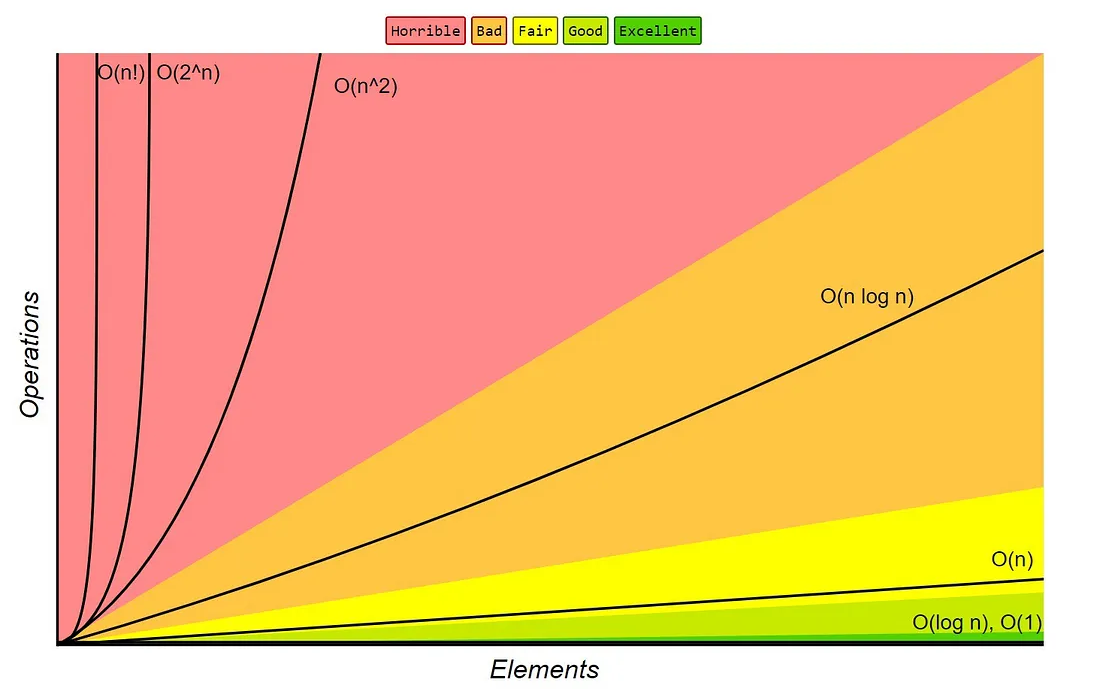
\includegraphics[width=0.6\textwidth]{./assets/images/Asymptotic Notations.png}
  \caption{Asymptotic Notation}
  \floatfoot{Big-O Complexity Analysis Chart from freeCodeCamp}
\end{figure}

\subsection{Big-O Notation}

The \textbf{\textit{big-O notation}} is used to describe the upper bound
on the growth rate of an algorithm as the input size approaches infinity.
It provides an upper limit on the worst-case time complexity of an algorithm.
The big-O notation is used to analyze the efficiency of an algorithm in terms
of the number of basic operations it performs.

\subsection{Omega Notation}

The \textbf{\textit{omega notation}} or \textbf{\textit{big-omega notation}}
is used to describe the lower bound on the growth rate of an algorithm as the
input size approaches infinity. It provides a lower limit on the best-case
time complexity of an algorithm. The omega notation is used to analyze the
efficiency of an algorithm in terms of the minimum number of basic operations
it performs.

\subsection{Theta Notation}

The \textbf{\textit{theta notation}} or \textbf{\textit{big-theta notation}}
is used to describe the tight bound on the growth rate of an algorithm as
the input size approaches infinity. It provides an upper and lower limit on
the time complexity of an algorithm. The theta notation is used to analyze
the efficiency of an algorithm in terms of the average number of basic
operations it performs.

\subsection{Complexity of an Algorithm}

The \textbf{\textit{complexity of an algorithm}} is a measure of the amount of time and
space required to execute the algorithm as a function of the input size. It is used
to analyze the efficiency of an algorithm and to compare different algorithms for
the same problem. The complexity of an algorithm is usually expressed using big-O
notation, which provides an upper bound on the growth rate of the algorithm as the
input size increases.

\subsubsection{Time Complexity}

The \textbf{\textit{time complexity}} of an algorithm is a measure of the amount of time
required to execute the algorithm as a function of the input size. It is used to
analyze the efficiency of an algorithm in terms of the number of basic operations
it performs. The time complexity of an algorithm is usually expressed using big-O
notation, which provides an upper bound on the growth rate of the algorithm as the
input size increases.

\paragraph{Constant Time Complexity ($O(1)$)}

An algorithm is said to have a \textbf{\textit{constant time complexity}} if the
execution time of the algorithm does not depend on the input size. It means
that the algorithm takes the same amount of time to execute regardless of
the input size. An example of an algorithm with constant time complexity is
accessing an element in an array using its index.

\begin{lstlisting}[language=C++, caption={Constant Time Complexity}]
int arr[5] = {1, 2, 3, 4, 5};
int x = arr[2]; // Accessing the element at index 2
\end{lstlisting}

\paragraph{Logarithmic Time Complexity ($O(\log n)$)}

An algorithm is said to have a \textbf{\textit{logarithmic time complexity}} if
the execution time of the algorithm grows logarithmically as the input size
increases. An example of an algorithm with logarithmic time complexity is
binary search, where the input size is halved at each step.

\begin{lstlisting}[language=C++, caption={Logarithmic Time Complexity}]
int binarySearch(int arr[], int n, int x) {
    int low = 0, high = n - 1;
    while (low <= high) {
        int mid = low + (high - low) / 2;
        if (arr[mid] == x) return mid;
        else if (arr[mid] < x) low = mid + 1;
        else high = mid - 1;
    }
    return -1;
}
\end{lstlisting}

\paragraph{Linear Time Complexity ($O(n)$)}

An algorithm is said to have a \textbf{\textit{linear time complexity}} if the
execution time of the algorithm grows linearly as the input size increases.
It means that the algorithm takes a constant amount of time to process each
element in the input. An example of an algorithm with linear time complexity
is traversing an array to find the maximum element.

\begin{lstlisting}[language=C++, caption={Linear Time Complexity}]
int findMax(int arr[], int n) {
    int max = arr[0];
    for (int i = 1; i < n; i++) {
        if (arr[i] > max) max = arr[i];
    }
    return max;
}
\end{lstlisting}

\paragraph{Linearithmic Time Complexity ($O(n \log n)$)}

An algorithm is said to have a \textbf{\textit{linearithmic time complexity}} if
the execution time of the algorithm grows linearithmically as the input size
increases. An example of an algorithm with linearithmic time complexity is
sorting an array using the merge sort algorithm.

\begin{lstlisting}[language=C++, caption={Linearithmic Time Complexity}]
void merge(int arr[], int l, int m, int r) {
    // Merge two subarrays of arr[]
    int i, j, k;
    int n1 = m - l + 1;
    int n2 = r - m;
    
    int *L = new int[n1];
    int *R = new int[n2];

    for (i = 0; i < n1; i++) L[i] = arr[l + i];
    for (j = 0; j < n2; j++) R[j] = arr[m + 1 + j];

    i = 0; j = 0; k = l;
    while (i < n1 && j < n2) {
        if (L[i] <= R[j]) arr[k++] = L[i++];
        else arr[k++] = R[j++];
    }

    while (i < n1) arr[k++] = L[i++];
    while (j < n2) arr[k++] = R[j++];
}

void mergeSort(int arr[], int l, int r) {
    if (l < r) {
        int m = l + (r - l) / 2;
        mergeSort(arr, l, m);
        mergeSort(arr, m + 1, r);
        merge(arr, l, m, r);
    }
}
\end{lstlisting}

\paragraph{Quadratic Time Complexity ($O(n^2)$)}

An algorithm is said to have a \textbf{\textit{quadratic time complexity}} if
the execution time of the algorithm grows quadratically as the input size
increases. It means that the time taken by the algorithm to process each
element in the input is proportional to the square of the input size. An
example of an algorithm with quadratic time complexity is the bubble sort
algorithm.

\begin{lstlisting}[language=C++, caption={Quadratic Time Complexity}]
void bubbleSort(int arr[], int n) {
    for (int i = 0; i < n - 1; i++) {
        for (int j = 0; j < n - i - 1; j++) {
            if (arr[j] > arr[j + 1]) {
                int temp = arr[j];
                arr[j] = arr[j + 1];
                arr[j + 1] = temp;
            }
        }
    }
}
\end{lstlisting}

Another common example of an algorithm with quadratic time complexity is
a nested loop that iterates over all pairs of elements in an array.

\paragraph{Exponential Time Complexity ($O(2^n)$)}

An algorithm is said to have an \textbf{\textit{exponential time complexity}} if
the execution time of the algorithm grows exponentially as the input size
increases. It means that the time taken by the algorithm increases
exponentially with each additional element in the input. An example of an
algorithm with exponential time complexity is the recursive Fibonacci
sequence algorithm.

\begin{lstlisting}[language=C++, caption={Exponential Time Complexity}]
int fibonacci(int n) {
    if (n <= 1) return n;
    return fibonacci(n - 1) + fibonacci(n - 2);
}
\end{lstlisting}

\paragraph{Factorial Time Complexity ($O(n!)$)}

An algorithm is said to have a \textbf{\textit{factorial time complexity}} if
the execution time of the algorithm grows factorially as the input size
increases. It means that the time taken by the algorithm increases
a factorial number of times with each additional element in the input.
An example of an algorithm with factorial time complexity is the
permutation algorithm that generates all possible permutations of a
set of elements.

\begin{lstlisting}[language=C++, caption={Factorial Time Complexity}]
void permute(string str, int l, int r) {
    if (l == r) cout << str << endl;
    else {
        for (int i = l; i <= r; i++) {
            swap(str[l], str[i]);
            permute(str, l + 1, r);
            swap(str[l], str[i]);
        }
    }
}
\end{lstlisting}

\subsubsection{Space Complexity}

The \textbf{\textit{space complexity}} of an algorithm is a measure of the amount
of memory required to execute the algorithm as a function of the input size. It
is used to analyze the efficiency of an algorithm in terms of the amount of
memory it uses. The space complexity of an algorithm is usually expressed using
big-O notation, which provides an upper bound on the amount of memory the
algorithm uses as the input size increases.

\paragraph{Constant Space Complexity ($O(1)$)}

An algorithm is said to have a \textbf{\textit{constant space complexity}} if
the amount of memory required to execute the algorithm does not depend on the
input size. It means that the algorithm uses a fixed amount of memory to
process the input. An example of an algorithm with constant space complexity
is swapping two variables without using a temporary variable.

\begin{lstlisting}[language=C++, caption={Constant Space Complexity}]
void swap(int &a, int &b) {
    a = a + b;
    b = a - b;
    a = a - b;
}
\end{lstlisting}

\paragraph{Linear Space Complexity ($O(n)$)}

An algorithm is said to have a \textbf{\textit{linear space complexity}} if the
amount of memory required to execute the algorithm grows linearly as the input
size increases. It means that the algorithm uses a memory space that is
proportional to the input size. An example of an algorithm with linear space
complexity is storing the elements of an array in a separate array in reverse
order.

\begin{lstlisting}[language=C++, caption={Linear Space Complexity}]
void reverseArray(int arr[], int n) {
    int start = 0, end = n - 1;
    while (start < end) {
        int temp = arr[start];
        arr[start] = arr[end];
        arr[end] = temp;
        start++;
        end--;
    }
}
\end{lstlisting}

\paragraph{Quadratic Space Complexity ($O(n^2)$)}

An algorithm is said to have a \textbf{\textit{quadratic space complexity}} if
the amount of memory required to execute the algorithm grows quadratically as
the input size increases. It means that the algorithm uses a memory space that
is proportional to the square of the input size. An example of an algorithm
with quadratic space complexity is storing all pairs of elements in an array
in a separate array.

\begin{lstlisting}[language=C++, caption={Quadratic Space Complexity}]
void allPairs(int arr[], int n) {
    vector<int> pairs(n * n);
    for (int i = 0; i < n; i++) {
        for (int j = 0; j < n; j++) {
            pairs[i * n + j] = arr[i] + arr[j];
        }
    }
}
\end{lstlisting}

\paragraph{Exponential Space Complexity ($O(2^n)$)}

An algorithm is said to have an \textbf{\textit{exponential space complexity}}
if the amount of memory required to execute the algorithm grows exponentially
as the input size increases. An example of an algorithm with exponential space
complexity is generating all subsets of a set of elements.

\begin{lstlisting}[language=C++, caption={Exponential Space Complexity}]
void generateSubsets(int arr[], int n) {
    for (int i = 0; i < (1 << n); i++) {
        for (int j = 0; j < n; j++) {
            if (i & (1 << j)) cout << arr[j] << " ";
        }
        cout << endl;
    }
}
\end{lstlisting}

\paragraph{Factorial Space Complexity ($O(n!)$)}

An algorithm is said to have a \textbf{\textit{factorial space complexity}} if
the amount of memory required to execute the algorithm grows factorially as
the input size increases. An example of an algorithm with factorial space
complexity is generating all permutations of a set of elements.

\begin{lstlisting}[language=C++, caption={Factorial Space Complexity}]
void permute(string str, int l, int r) {
    if (l == r) cout << str << endl;
    else {
        for (int i = l; i <= r; i++) {
            swap(str[l], str[i]);
            permute(str, l + 1, r);
            swap(str[l], str[i]);
        }
    }
}
\end{lstlisting}

\section{Summary}

In this chapter, we introduced the fundamental concepts of data structures
and algorithms. We discussed the importance of data structures and algorithms
in computer science and software engineering. We also covered some basic
terminologies related to data structures and algorithms, such as data, data
object, data type, abstract data type, and complexity of an algorithm. We
introduced the concept of asymptotic notations, such as big-O notation, omega
notation, and theta notation, and discussed the time complexity of algorithms
in terms of big-O notation. We covered common time complexity ranges from best
to worst performance, such as constant time complexity, logarithmic time
complexity, linear time complexity, linearithmic time complexity, quadratic
time complexity, exponential time complexity, and factorial time complexity.

\section{Coding Exercises}

\begin{enumerate}
    \item Implement a C++ program that demonstrates the primitive data types.
    \begin{enumerate}
        \item Declare and initialize variables of the following different data types.
        \begin{enumerate}
            \item Integer
            \item Float
            \item Double
            \item Character
            \item Boolean
        \end{enumerate}
        \item Print the values of the variables to the console.
    \end{enumerate}
    \item Implement a C++ program to find the maximum element in an array
    using linear time complexity.
    \begin{enumerate}
        \item Declare an array of integers.
        \begin{align*}
            \text{int arr[6];}
        \end{align*}
        \item Initialize the array with random values.
        \begin{align*}
            \text{arr[6] = \{19, 10, 8, 17, 9, 15\};}
        \end{align*}
        \item Find the maximum element in the array.
        \item Print the maximum element to the console.
        \begin{quote}
            Output: 19
        \end{quote}
        \item Determine the \textbf{time complexity} and \textbf{space complexity} of the program.
    \end{enumerate}
    \item Implement a C++ program to find the sum of all elements in an array
    using linear time complexity.
    \begin{enumerate}
        \item Declare an array of integers.
        \begin{align*}
            \text{int arr[6];}
        \end{align*}
        \item Initialize the array with random values.
        \begin{align*}
            \text{arr[6] = \{19, 10, 8, 17, 9, 15\};}
        \end{align*}
        \item Find the sum of all elements in the array.
        \item Print the sum to the console.
        \begin{quote}
            Output: 78
        \end{quote}
        \item Determine the \textbf{time complexity} and \textbf{space complexity} of the program.
    \end{enumerate}
    % \item Implement a C++ program to reverse an array in place using linear
    % time complexity.
    % \item Implement a C++ program to sort an array using the bubble sort
    % algorithm with quadratic time complexity.
    % \item Implement a C++ program to generate all subsets of a set of elements
    % using exponential space complexity.
    % \item Implement a C++ program to generate all permutations of a set of
    % elements using factorial space complexity.
\end{enumerate}

%%%%%%%%%%%%%%%%%%%%%%%%%%%%%%%%%%%%
%%%%%~ NEW CHAPTER STARTS HERE %%%%%
%%%%%%%%%%%%%%%%%%%%%%%%%%%%%%%%%%%%
\chapter{Arrays and Linked Lists}

\section{Introduction}

Some of the most basic and fundamental data structures in computer science
are arrays and linked lists. These data structures are used to store and
manipulate collections of elements in a computer program. In this chapter,
we will discuss the properties, operations, and complexity analysis of
arrays and linked lists.

\section{Arrays}

An \textbf{\textit{array}} is a collection of elements of the same data type
that are stored in contiguous memory locations. It is used to store multiple
values of the same type under a single name. The elements of an array can be
accessed using an index value. In C++, arrays are zero-indexed, which means
the first element is at index 0. Arrays also have a fixed size that is
specified at the time of declaration.

\begin{figure}[h]
    \centering
    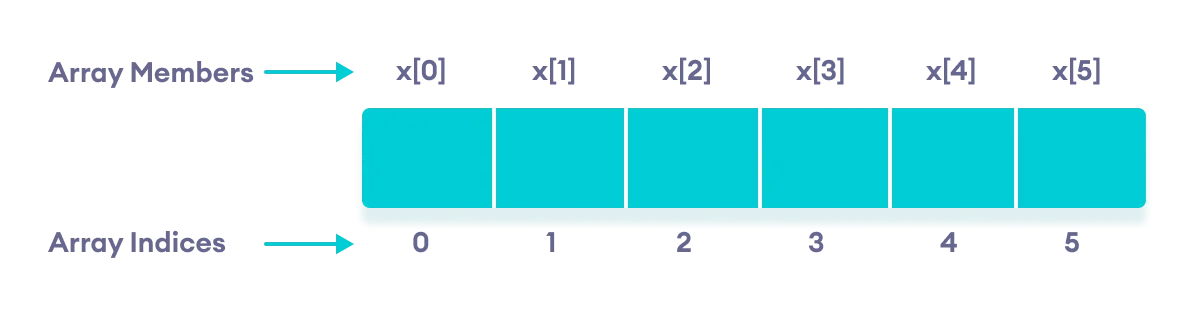
\includegraphics[width=0.8\textwidth]{./assets/images/cpp-array-declaration_0.png}
    \caption{Elements of an array in C++}
    \floatfoot{Elements of an array in C++ from Programiz}
    \label{fig:array-elements}
\end{figure}

Figure \ref{fig:array-elements} shows the the visual representation of the
elements of an array in C++. It shows the array members and indices.

% Code example for array declaration
\begin{lstlisting}[language=C++, caption={Array Declaration}]
// array.cpp
int main() {
    int arr[6];
    return 0;
}
\end{lstlisting}

The above code snippet declares an array named \texttt{arr} of size 6 that
can store 6 integer values. The elements of the array are accessed using
index values from 0 to 5 as shown in Figure \ref{fig:array-elements}.

% Code for assigning values to array elements
\begin{lstlisting}[language=C++, caption={Assigning Values to Array Elements}]
// array_assign.cpp
int main() {
    int arr[6];
    arr[0] = 19;
    arr[1] = 10;
    arr[2] = 8;
    return 0;
}
\end{lstlisting}

The above code snippet assigns values to the elements of the array \texttt{arr}
at index 0, 1, and 2. The elements of the array can be accessed and modified
using their index values. Array elements that are not explicitly initialized
are assigned default values based on their data type. For example, integer
elements are initialized to 0.

% Insert image for array initialization
\begin{figure}[h]
  \centering
  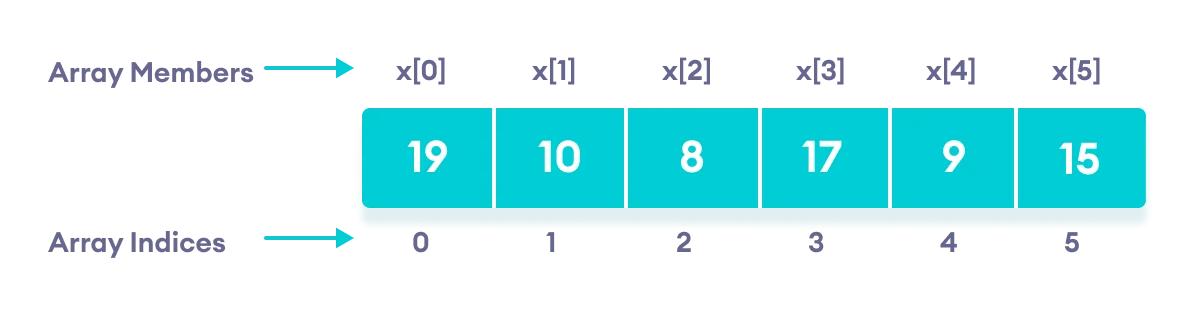
\includegraphics[width=0.8\textwidth]{./assets/images/cpp-array-initialization_0.png}
  \caption{Initializing Array Elements}
    \floatfoot{Initializing Array Elements from Programiz}
    \label{fig:array-initialization}
\end{figure}

Figure \ref{fig:array-initialization} shows the code for initializing array
elements in C++. The array elements are initialized using curly braces
\texttt{\{\}} with the values separated by commas. When the size of the array
is specified, the number of elements in the initialization list must match
the size of the array. If the size of the array is not specified, the size
is automatically determined based on the number of elements in the array
during initialization.

% Code for initializing array elements
\begin{lstlisting}[language=C++, caption={Initializing Array Elements}]
int main() {
    int arr[6] = {19, 10, 8, 17, 9, 15};
    return 0;
}
\end{lstlisting}

The above code snippet initializes the elements of the array \texttt{arr} with
the values 19, 10, 8, 17, 9, and 15. The size of the array is specified as 6,
and the number of elements in the initialization list matches the size of the
array.

% Another code example for array initialization with unspecified size
\begin{lstlisting}[language=C++, caption={Initializing Array Elements with Unspecified Size}]
int main() {
    int arr[] = {19, 10, 8, 17, 9, 15};
    return 0;
}
\end{lstlisting}

The above code snippet initializes the elements of the array \texttt{arr} with
the values 19, 10, 8, 17, 9, and 15. The size of the array is not specified
and is automatically determined based on the number of elements in the
initialization list.

% Figure for array initialization with empty members
\begin{figure}[h]
  \centering
  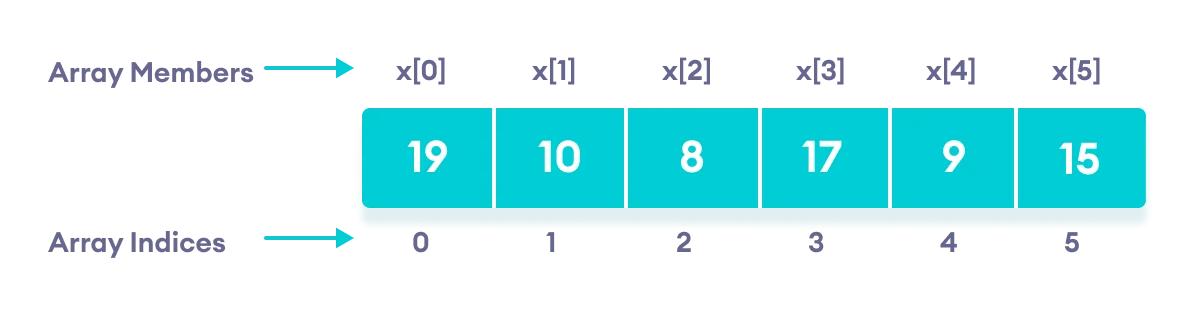
\includegraphics[width=0.8\textwidth]{./assets/images/cpp-array-initialization_0.png}
  \caption{Initializing Array Elements with Empty Members}
    \floatfoot{Initializing Array Elements with Empty Members from Programiz}
    \label{fig:array-initialization-empty}
\end{figure}

Figure \ref{fig:array-initialization-empty} shows the code for initializing
array elements with empty members in C++. The array elements are initialized
using curly braces \texttt{\{\}} with empty members. Empty members only
appear at the end of the initialization list and are assigned default values
based on their data type. For example, integer elements are initialized to 0.

% Code for initializing array elements with empty members
\begin{lstlisting}[language=C++, caption={Initializing Array Elements with Empty Members}]
int main() {
    int arr[6] = {19, 10, 8};
    return 0;
}
\end{lstlisting}

The above code snippet initializes the first three elements of the array
\texttt{arr} with the values 19, 10, and 8. The remaining elements of the
array are initialized to 0, which is the default value for integer elements.

\subsection{Types of Arrays}

There are two main types of arrays in C++: one-dimensional arrays and
multi-dimensional arrays.

\subsubsection{One-dimensional Array}

A \textbf{\textit{one-dimensional array}} is a collection of elements of the
same data type that are stored in a single row. It is the most common type
of array used in computer programming. The elements of a one-dimensional array
are accessed using a single index value.

% Figure for one-dimensional array
\begin{figure}[h]
  \centering
  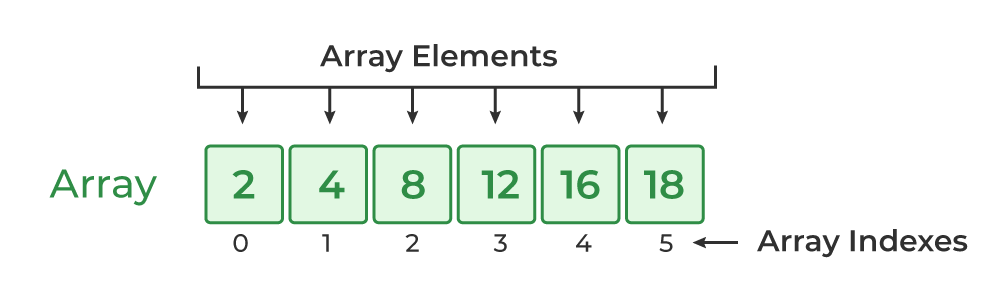
\includegraphics[width=0.8\textwidth]{./assets/images/Arrays-in-C.png}
  \caption{One-dimensional Array in C++}
    \floatfoot{One-dimensional Array in C++ from GeekforGeeks}
    \label{fig:one-dimensional-array}
\end{figure} 

Figure \ref{fig:one-dimensional-array} shows the visual representation of a
one-dimensional array in C++. As shown in the figure, the elements of the
array are stored in a single row, and each element is accessed using a single
index value.

% Code example for one-dimensional array
\begin{lstlisting}[language=C++, caption={One-dimensional Array}]
int main() {
    int arr[6] = {2, 4, 8, 12, 16, 18};
    return 0;
}
\end{lstlisting}

The above code snippet declares and initializes a one-dimensional array named
\texttt{arr} with 6 integer elements. A one-dimensional array only has one
set of square brackets \texttt{[]}. One set of square brackets signifies that
the array is one-dimensional.

\subsubsection{Multi-dimensional Array}

A \textbf{\textit{multi-dimensional array}} is a collection of elements of the
same data type that are stored in multiple rows and columns. It is used to
store data in a tabular format. The elements of a multi-dimensional array are
accessed using multiple index values.

% Figure for two-dimensional array
\begin{figure}[h]
  \centering
  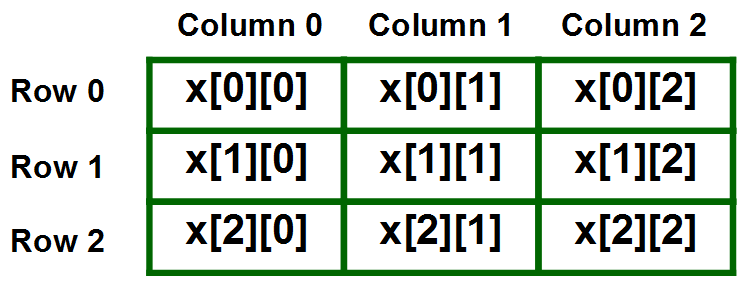
\includegraphics[width=0.8\textwidth]{./assets/images/two-d.png}
  \caption{Two-dimensional Array in C++}
    \floatfoot{Two-dimensional Array in C++ from GeekforGeeks}
    \label{fig:two-dimensional-array}
\end{figure}

Figure \ref{fig:two-dimensional-array} shows the visual representation of a
two-dimensional array in C++. As shown in the figure, the elements of the
array are stored in multiple rows and columns, and each element is accessed
using two index values. The number of elements in a two-dimensional array is
determined by the number of rows and columns.

% Code example for two-dimensional array
\begin{lstlisting}[language=C++, caption={Two-dimensional Array}]
int main() {
    int arr[3][4] = {
        {1, 2, 3, 4},
        {5, 6, 7, 8},
        {9, 10, 11, 12}
    };
    return 0;
}
\end{lstlisting}

The above code snippet declares and initializes a two-dimensional array named
\texttt{arr} with 3 rows and 3 columns. A two-dimensional array has two sets
of square brackets \texttt{[][]}. Two sets of square brackets signify that the
array is two-dimensional. The number of rows and columns in a two-dimensional
array is specified within the square brackets. The first set of square brackets
specifies the number of rows, and the second set of square brackets specifies
the number of columns. Thus, in the above example, the array \texttt{arr} has
3 rows and 4 columns.

% Code With empty members
\begin{lstlisting}[language=C++, caption={Two-dimensional Array with Empty Members}]
int main() {
    int arr[3][4] = {
        {1, 2},
        {5, 6, 7},
        {9}
    };
    return 0;
}
\end{lstlisting}

The above code snippet initializes the elements of the two-dimensional array
\texttt{arr} with empty members. The first row of the array has 2 elements,
the second row has 3 elements, and the third row has 1 element. The remaining
elements of the array are initialized to 0, which is the default value for
integer elements.

\subsection{Array Operations}

Arrays support various operations such as insertion, deletion, and searching
of elements. These operations are essential for manipulating the elements of
an array and performing various tasks in a computer program.

\subsubsection{Insertion}

The \textbf{\textit{insertion}} operation is used to add an element to an array
at a specific position. The element is inserted at the specified index, and
the existing elements are shifted to accommodate the new element.

% TikZ diagram for array insertion
\begin{figure}[h]
    \centering
    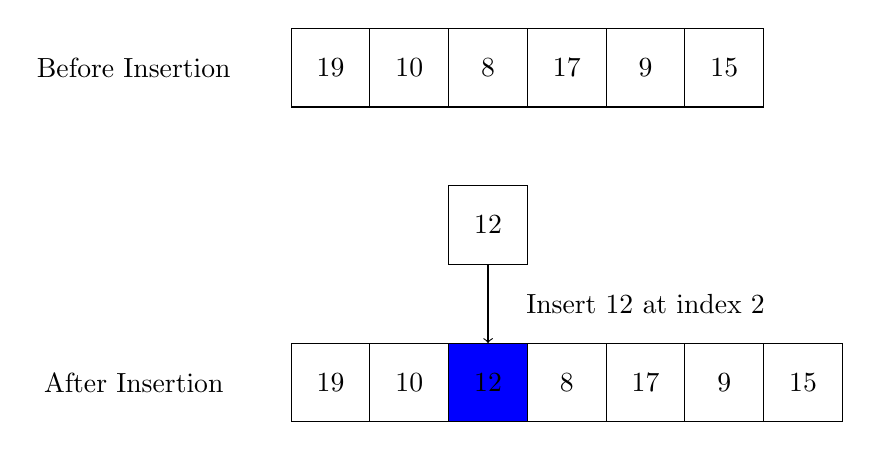
\begin{tikzpicture}
        % Make a one dimensional grid with 6 elements
        \draw (0, 0) grid (6, 1);
        % Fill the grid with the elements
        \foreach \x/\y in {
            0/19, 1/10, 2/8, 3/17, 4/9, 5/15
        }
        \node at (\x + 0.5, 0.5) {\y};
        \node at (-2, 0.5) {Before Insertion};

        % Insert a new element at index 2
        \draw (2, -1) rectangle (3, -2);
        \node at (2.5, -1.5) {12};

        % Draw Arrow with label "Insert"
        \draw[->] (2.5, -2) -- (2.5, -3);
        \node at (4.5, -2.5) {Insert 12 at index 2};
        
        % Create a new grid with the inserted element
        \draw (0, -4) grid (7, -3);
        % Color the grid with inserted element
        \draw[fill=blue] (2, -4) rectangle (3, -3);

        \foreach \x/\y in {
            0/19, 1/10, 2/12, 3/8, 4/17, 5/9, 6/15
        }
        \node at (\x + 0.5, -3.5) {\y};
        \node at (-2, -3.5) {After Insertion};
    \end{tikzpicture}
    \caption{Array Insertion}
    \label{fig:array-insertion}
\end{figure}

Figure \ref{fig:array-insertion} shows the visual representation of the
insertion operation in an array. The element 12 is inserted at index 2 of
the array, and the existing elements are shifted to accommodate the new
element.

% Code example for array insertion
\begin{lstlisting}[language=C++, caption={Array Insertion}, label={lst:array-insertion}]
int main() {
    int arr[100] = {19, 10, 8, 17, 9, 15};
    int n = 6;
    int index = 2;
    int value = 12;

    for (int i = n - 1; i >= index; i--) {
        arr[i + 1] = arr[i];
    }
    arr[index] = value;
    n++;

    return 0;
}
\end{lstlisting}

Code \ref{lst:array-insertion} shows the code for inserting an element
into an array in C++. The code snippet declares an array \texttt{arr} of size
100 and initializes it with 6 elements. It then inserts the element 12 at
index 2 of the array and shifts the existing elements to accommodate the new
element.

\subsubsection{Deletion}

The \textbf{\textit{deletion}} operation is used to remove an element from an
array at a specific position. The element is deleted from the specified index,
and the remaining elements are shifted to fill the gap created by the deletion.

% TikZ diagram for array deletion
\begin{figure}[h]
    \centering
    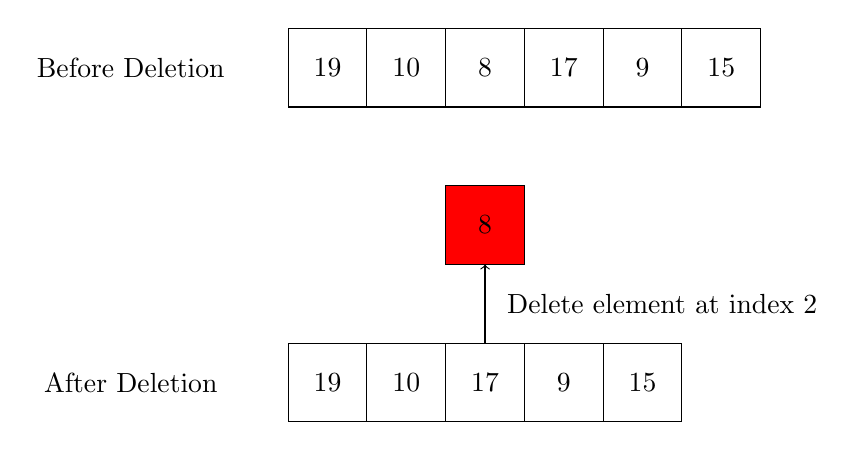
\begin{tikzpicture}
        % Make a one dimensional grid with 6 elements
        \draw (0, 0) grid (6, 1);
        % Fill the grid with the elements
        \foreach \x/\y in {
            0/19, 1/10, 2/8, 3/17, 4/9, 5/15
        }
        \node at (\x + 0.5, 0.5) {\y};
        \node at (-2, 0.5) {Before Deletion};

        % Delete the element at index 2
        \draw[fill=red] (2, -1) rectangle (3, -2);
        \node at (2.5, -1.5) {8};

        % Draw Arrow with label "Delete"
        \draw[->] (2.5, -3) -- (2.5, -2);
        \node at (4.75, -2.5) {Delete element at index 2};
        
        % Create a new grid with the deleted element
        \draw (0, -4) grid (5, -3);

        \foreach \x/\y in {
            0/19, 1/10, 2/17, 3/9, 4/15
        }
        \node at (\x + 0.5, -3.5) {\y};
        \node at (-2, -3.5) {After Deletion};
    \end{tikzpicture}
    \caption{Array Deletion}
    \label{fig:array-deletion}
\end{figure}


Figure \ref{fig:array-deletion} shows the visual representation of the deletion
operation in an array. The element 8 is deleted from index 2 of the array, and
the remaining elements are shifted to fill the gap created by the deletion.

% Code example for array deletion
\begin{lstlisting}[language=C++, caption={Array Deletion}, label={lst:array-deletion}]
int main() {
    int arr[100] = {19, 10, 8, 17, 9, 15};
    int n = 6;
    int index = 2;

    for (int i = index; i < n - 1; i++) {
        arr[i] = arr[i + 1];
    }
    n--;

    return 0;
}
\end{lstlisting}

Code \ref{lst:array-deletion} shows the code for deleting an element from an
array in C++. The code snippet declares an array \texttt{arr} of size 100 and
initializes it with 6 elements. It then deletes the element at index 2 of the
array and shifts the remaining elements to fill the gap created by the deletion.

\subsubsection{Searching}

The \textbf{\textit{searching}} operation is used to find the position of an
element in an array. The element is searched for in the array, and the index
of the element is returned if it is found. If the element is not found, a
special value such as -1 is returned to indicate that the element is not
present in the array.

% TikZ diagram for array searching
\begin{figure}[h]
    \centering
    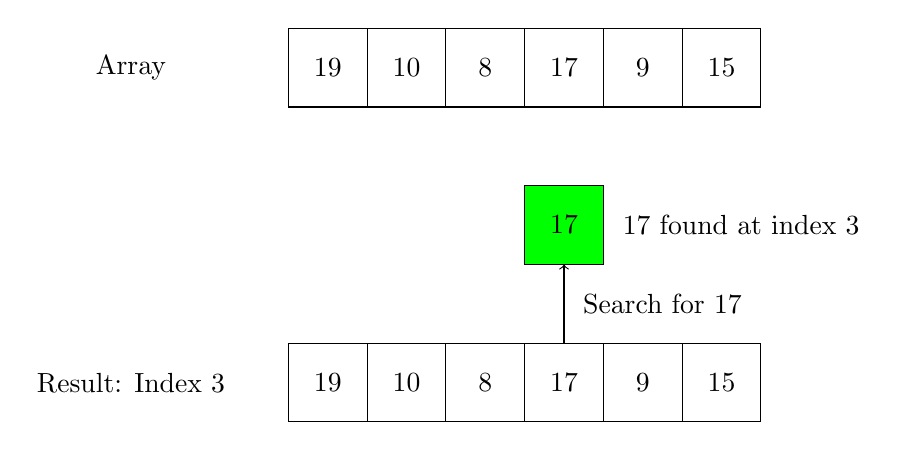
\begin{tikzpicture}
        % Make a one dimensional grid with 6 elements
        \draw (0, 0) grid (6, 1);
        % Fill the grid with the elements
        \foreach \x/\y in {
            0/19, 1/10, 2/8, 3/17, 4/9, 5/15
        }
        \node at (\x + 0.5, 0.5) {\y};
        \node at (-2, 0.5) {Array};

        % Search for the element 17
        \draw[fill=green] (3, -1) rectangle (4, -2);
        \node at (3.5, -1.5) {17};

        % Draw Arrow with label "Search"
        \draw[->] (3.5, -3) -- (3.5, -2);
        \node at (4.75, -2.5) {Search for 17};
        \node at (5.75, -1.5) {17 found at index 3};

        % Create a new grid with the searched element
        \draw (0, -4) grid (6, -3);

        \foreach \x/\y in {
            0/19, 1/10, 2/8, 3/17, 4/9, 5/15
        }
        \node at (\x + 0.5, -3.5) {\y};
        \node at (-2, -3.5) {Result: Index 3};
    \end{tikzpicture}
    \caption{Array Searching}
    \label{fig:array-searching}
\end{figure}

Figure \ref{fig:array-searching} shows the visual representation of the
searching operation in an array. The element 17 is searched for in the array,
and the index of the element is returned if it is found. In this case, the
element 17 is found at index 3 of the array.

% Code example for array searching
\begin{lstlisting}[language=C++, caption={Array Searching}, label={lst:array-searching}]
int main() {
    int arr[100] = {19, 10, 8, 17, 9, 15};
    int n = 6;
    int value = 17;
    int index = -1;

    for (int i = 0; i < n; i++) {
        if (arr[i] == value) {
            index = i;
            break;
        }
    }

    return 0;
}
\end{lstlisting}

Code \ref{lst:array-searching} shows the code for searching an element in an
array in C++. The code snippet declares an array \texttt{arr} of size 100 and
initializes it with 6 elements. It then searches for the element 17 in the
array and returns the index of the element if it is found. In this case, the
element 17 is found at index 3 of the array. The searching algorithm used in
the example is a linear search algorithm.

% \subsection{Complexity Analysis of Arrays}

\section{Linked Lists}

A \textbf{\textit{linked list}} is a data structure that consists of a sequence
of elements called nodes. A node contains a data part and a reference part that
points to the next or previous node in the sequence. Linked lists are used to
store and manipulate collections of elements in a computer program. Unlike
arrays, linked lists do not require contiguous memory locations, and the size
of a linked list can grow or shrink dynamically.

\subsection{Types of Linked Lists}

\subsubsection{Singly Linked List}

A \textbf{\textit{singly linked list}} is a type of linked list in which each
node contains a data part and a next part that points to the next node in the
sequence. The last node in the list points to a special value called NULL to
indicate the end of the list.

% TikZ diagram for singly linked list
\begin{figure}[h]
    \centering
    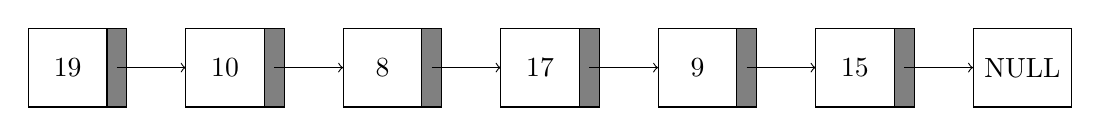
\begin{tikzpicture}
        % Draw the nodes of the singly linked list
        \draw (0, 0) rectangle (1, 1);
        \node at (0.5, 0.5) {19};
        \draw[fill=gray] (1, 1) rectangle (1.25, 0);

        \draw (2, 0) rectangle (3, 1);
        \node at (2.5, 0.5) {10};
        \draw[fill=gray] (3, 1) rectangle (3.25, 0);

        \draw (4, 0) rectangle (5, 1);
        \node at (4.5, 0.5) {8};
        \draw[fill=gray] (5, 1) rectangle (5.25, 0);

        \draw (6, 0) rectangle (7, 1);
        \node at (6.5, 0.5) {17};
        \draw[fill=gray] (7, 1) rectangle (7.25, 0);

        \draw (8, 0) rectangle (9, 1);
        \node at (8.5, 0.5) {9};
        \draw[fill=gray] (9, 1) rectangle (9.25, 0);

        \draw (10, 0) rectangle (11, 1);
        \node at (10.5, 0.5) {15};
        \draw[fill=gray] (11, 1) rectangle (11.25, 0);

        \draw (12, 0) rectangle (13.25, 1);
        \node at (12.625, 0.5) {NULL};

        % Draw the arrows between the nodes
        \draw[->] (1.125, 0.5) -- (2, 0.5);
        \draw[->] (3.125, 0.5) -- (4, 0.5);
        \draw[->] (5.125, 0.5) -- (6, 0.5);
        \draw[->] (7.125, 0.5) -- (8, 0.5);
        \draw[->] (9.125, 0.5) -- (10, 0.5);
        \draw[->] (11.125, 0.5) -- (12, 0.5);
    \end{tikzpicture}
    \caption{Singly Linked List}
    \label{fig:singly-linked-list}
\end{figure}

Figure \ref{fig:singly-linked-list} shows the visual representation of a singly
linked list. The linked list contains nodes with data values 19, 10, 8, 17, 9,
and 15. Each node points to the next node in the sequence, and the last node
points to NULL to indicate the end of the list.

% Code example for singly linked list
\begin{lstlisting}[language=C++, caption={Singly Linked List}, label={lst:singly-linked-list}]
struct Node {
    int data;
    Node *next;
    
    Node(int data) {
        this->data = data;
        this->next = NULL;
    }
};

int main() {
    Node *first = new Node(19);
    Node *second = new Node(10);
    Node *third = new Node(8);
    Node *fourth = new Node(17);
    Node *fifth = new Node(9);
    Node *sixth = new Node(15);

    Node *head = first;

    first->next = second;
    second->next = third;
    third->next = fourth;
    fourth->next = fifth;
    fifth->next = sixth;

    return 0;
}
\end{lstlisting}

Code \ref{lst:singly-linked-list} shows the code for creating a singly linked
list in C++. The code snippet defines a structure \texttt{Node} that contains
a data part and a next part that points to the next node in the sequence. It
then creates a linked list with nodes containing data values 19, 10, 8, 17, 9,
and 15. Each node points to the next node in the sequence, and the last node
points to NULL to indicate the end of the list.

\subsubsection{Doubly Linked List}

A \textbf{\textit{doubly linked list}} is a type of linked list in which each
node contains a data part, a next part that points to the next node in the
sequence, and a previous part that points to the previous node in the sequence.
The first node in the list points to NULL in the previous part, and the last
node in the list points to NULL in the next part.

% TikZ diagram for doubly linked list
\begin{figure}[h]
    \centering
    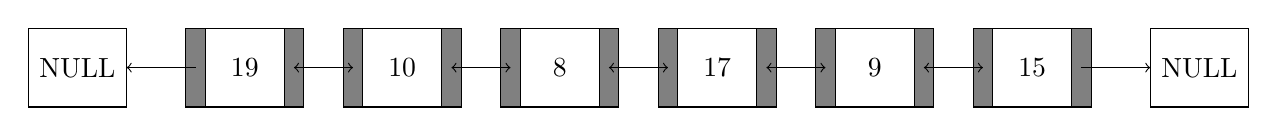
\begin{tikzpicture}
        % Draw the nodes of the doubly linked list
        \draw (-1, 0) rectangle (-2.25, 1);
        \node at (-1.625, 0.5) {NULL};

        \draw (0, 0) rectangle (1, 1);
        \node at (0.5, 0.5) {19};
        \draw[fill=gray] (1, 1) rectangle (1.25, 0);
        \draw[fill=gray] (-0.25, 1) rectangle (0, 0);

        \draw (2, 0) rectangle (3, 1);
        \node at (2.5, 0.5) {10};
        \draw[fill=gray] (3, 1) rectangle (3.25, 0);
        \draw[fill=gray] (1.75, 1) rectangle (2, 0);

        \draw (4, 0) rectangle (5, 1);
        \node at (4.5, 0.5) {8};
        \draw[fill=gray] (5, 1) rectangle (5.25, 0);
        \draw[fill=gray] (3.75, 1) rectangle (4, 0);

        \draw (6, 0) rectangle (7, 1);
        \node at (6.5, 0.5) {17};
        \draw[fill=gray] (7, 1) rectangle (7.25, 0);
        \draw[fill=gray] (5.75, 1) rectangle (6, 0);

        \draw (8, 0) rectangle (9, 1);
        \node at (8.5, 0.5) {9};
        \draw[fill=gray] (9, 1) rectangle (9.25, 0);
        \draw[fill=gray] (7.75, 1) rectangle (8, 0);

        \draw (10, 0) rectangle (11, 1);
        \node at (10.5, 0.5) {15};
        \draw[fill=gray] (11, 1) rectangle (11.25, 0);
        \draw[fill=gray] (9.75, 1) rectangle (10, 0);

        \draw (12, 0) rectangle (13.25, 1);
        \node at (12.625, 0.5) {NULL};

        % Draw the arrows between the nodes
        \draw[<-] (-1, 0.5) -- (-0.125, 0.5);
        \draw[<->] (1.125, 0.5) -- (1.875, 0.5);
        \draw[<->] (3.125, 0.5) -- (3.875, 0.5);
        \draw[<->] (5.125, 0.5) -- (5.875, 0.5);
        \draw[<->] (7.125, 0.5) -- (7.875, 0.5);
        \draw[<->] (9.125, 0.5) -- (9.875, 0.5);
        \draw[->] (11.125, 0.5) -- (12, 0.5);
    \end{tikzpicture}
    \caption{Doubly Linked List}
    \label{fig:doubly-linked-list}
\end{figure}

Figure \ref{fig:doubly-linked-list} shows the visual representation of a doubly
linked list. The linked list contains nodes with data values 19, 10, 8, 17, 9,
and 15. Each node points to the next and previous nodes in the sequence, and
the first and last nodes point to NULL to indicate the end of the list.

% Code example for doubly linked list
\begin{lstlisting}[language=C++, caption={Doubly Linked List}, label={lst:doubly-linked-list}]
struct Node {
    int data;
    Node *next;
    Node *prev;
    
    Node(int data) {
        this->data = data;
        this->next = NULL;
        this->prev = NULL;
    }
};

int main() {
    Node *first = new Node(19);
    Node *second = new Node(10);
    Node *third = new Node(8);
    Node *fourth = new Node(17);
    Node *fifth = new Node(9);
    Node *sixth = new Node(15);

    Node *head = first;

    first->next = second;
    second->next = third;
    third->next = fourth;
    fourth->next = fifth;
    fifth->next = sixth;
    
    second->prev = first;
    third->prev = second;
    fourth->prev = third;
    fifth->prev = fourth;
    sixth->prev = fifth;

    return 0;
}
\end{lstlisting}

Code \ref{lst:doubly-linked-list} shows the code for creating a doubly linked
list in C++. The code snippet defines a structure \texttt{Node} that contains
a data part, a next part that points to the next node in the sequence, and a
previous part that points to the previous node in the sequence. It then creates
a linked list with nodes containing data values 19, 10, 8, 17, 9, and 15. Each
node points to the next and previous nodes in the sequence, and the first and
last nodes point to NULL to indicate the end of the list.

\subsubsection{Circular Linked List}

A \textbf{\textit{circular linked list}} is a type of linked list in which the
last node in the list points back to the first node, forming a circular loop.
This allows traversal of the list in a circular manner, starting from any node
in the list.

% TikZ diagram for circular linked list
\begin{figure}[h]
    \centering
    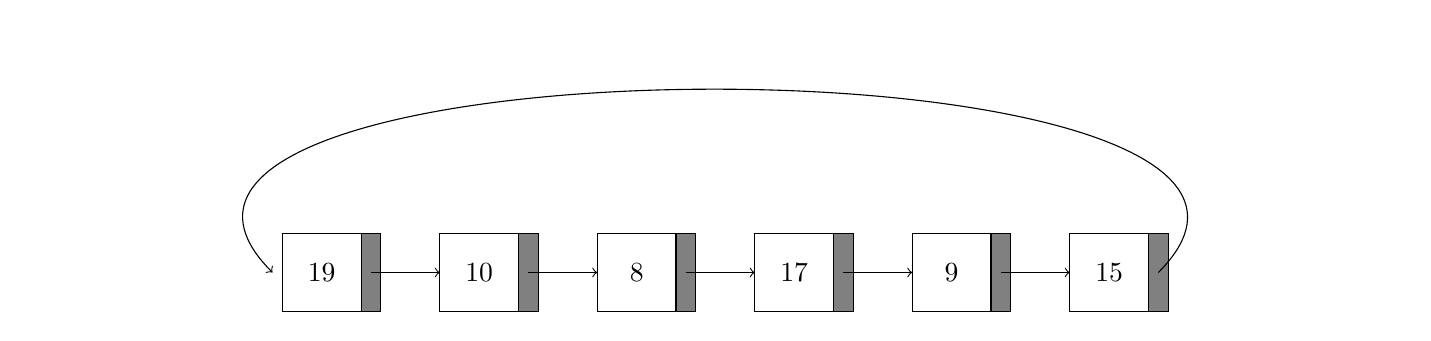
\begin{tikzpicture}
        % Draw the nodes of the circular linked list
        \draw (0, 0) rectangle (1, 1);
        \node at (0.5, 0.5) {19};
        \draw[fill=gray] (1, 1) rectangle (1.25, 0);

        \draw (2, 0) rectangle (3, 1);
        \node at (2.5, 0.5) {10};
        \draw[fill=gray] (3, 1) rectangle (3.25, 0);

        \draw (4, 0) rectangle (5, 1);
        \node at (4.5, 0.5) {8};
        \draw[fill=gray] (5, 1) rectangle (5.25, 0);

        \draw (6, 0) rectangle (7, 1);
        \node at (6.5, 0.5) {17};
        \draw[fill=gray] (7, 1) rectangle (7.25, 0);

        \draw (8, 0) rectangle (9, 1);
        \node at (8.5, 0.5) {9};
        \draw[fill=gray] (9, 1) rectangle (9.25, 0);

        \draw (10, 0) rectangle (11, 1);
        \node at (10.5, 0.5) {15};
        \draw[fill=gray] (11, 1) rectangle (11.25, 0);

        % Draw the arrows between the nodes
        \draw[->] (1.125, 0.5) -- (2, 0.5);
        \draw[->] (3.125, 0.5) -- (4, 0.5);
        \draw[->] (5.125, 0.5) -- (6, 0.5);
        \draw[->] (7.125, 0.5) -- (8, 0.5);
        \draw[->] (9.125, 0.5) -- (10, 0.5);

        % Add Curved Arrow from last node to first node
        \draw[->] (11.125, 0.5) to [out=45, in=135] (-0.125, 0.5);
    \end{tikzpicture}
    \caption{Circular Linked List}
    \label{fig:circular-linked-list}
\end{figure}

Figure \ref{fig:circular-linked-list} shows the visual representation of a
circular linked list. The linked list contains nodes with data values 19, 10,
8, 17, 9, and 15. Each node points to the next node in the sequence, and the
last node points back to the first node, forming a circular loop.

% Code example for circular linked list
\begin{lstlisting}[language=C++, caption={Circular Linked List}, label={lst:circular-linked-list}]
struct Node {
    int data;
    Node *next;
    
    Node(int data) {
        this->data = data;
        this->next = NULL;
    }
};

int main() {
    Node *first = new Node(19);
    Node *second = new Node(10);
    Node *third = new Node(8);
    Node *fourth = new Node(17);
    Node *fifth = new Node(9);
    Node *sixth = new Node(15);

    Node *head = first;

    first->next = second;
    second->next = third;
    third->next = fourth;
    fourth->next = fifth;
    fifth->next = sixth;
    sixth->next = head;

    return 0;
}
\end{lstlisting}

Code \ref{lst:circular-linked-list} shows the code for creating a circular
linked list in C++. The code snippet defines a structure \texttt{Node} that
contains a data part and a next part that points to the next node in the
sequence. It then creates a linked list with nodes containing data values 19,
10, 8, 17, 9, and 15. Each node points to the next node in the sequence, and
the last node points back to the first node, forming a circular loop.

\subsubsection{Doubly Circular Linked List}

A \textbf{\textit{doubly circular linked list}} is a type of linked list in
which each node contains a data part, a next part that points to the next node
in the sequence, and a previous part that points to the previous node in the
sequence. The first node in the list points to the last node in the previous
part, and the last node in the list points to the first node in the next part,
forming a circular loop.

% TikZ diagram for doubly circular linked list
\begin{figure}[h]
    \centering
    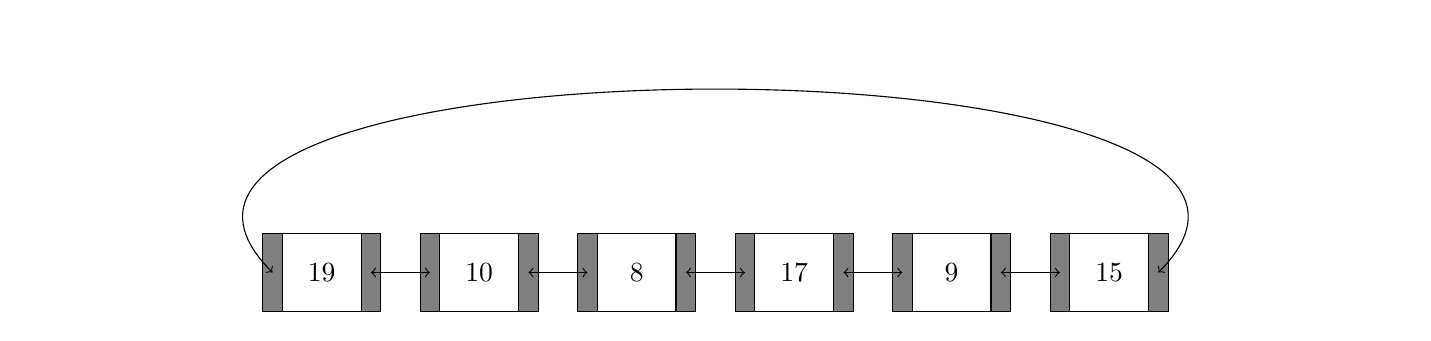
\begin{tikzpicture}
        % Draw the nodes of the doubly circular linked list
        \draw (0, 0) rectangle (1, 1);
        \node at (0.5, 0.5) {19};
        \draw[fill=gray] (1, 1) rectangle (1.25, 0);
        \draw[fill=gray] (-0.25, 1) rectangle (0, 0);

        \draw (2, 0) rectangle (3, 1);
        \node at (2.5, 0.5) {10};
        \draw[fill=gray] (3, 1) rectangle (3.25, 0);
        \draw[fill=gray] (1.75, 1) rectangle (2, 0);

        \draw (4, 0) rectangle (5, 1);
        \node at (4.5, 0.5) {8};
        \draw[fill=gray] (5, 1) rectangle (5.25, 0);
        \draw[fill=gray] (3.75, 1) rectangle (4, 0);

        \draw (6, 0) rectangle (7, 1);
        \node at (6.5, 0.5) {17};
        \draw[fill=gray] (7, 1) rectangle (7.25, 0);
        \draw[fill=gray] (5.75, 1) rectangle (6, 0);

        \draw (8, 0) rectangle (9, 1);
        \node at (8.5, 0.5) {9};
        \draw[fill=gray] (9, 1) rectangle (9.25, 0);
        \draw[fill=gray] (7.75, 1) rectangle (8, 0);

        \draw (10, 0) rectangle (11, 1);
        \node at (10.5, 0.5) {15};
        \draw[fill=gray] (11, 1) rectangle (11.25, 0);
        \draw[fill=gray] (9.75, 1) rectangle (10, 0);

        % Draw the arrows between the nodes
        \draw[<->] (1.125, 0.5) -- (1.875, 0.5);
        \draw[<->] (3.125, 0.5) -- (3.875, 0.5);
        \draw[<->] (5.125, 0.5) -- (5.875, 0.5);
        \draw[<->] (7.125, 0.5) -- (7.875, 0.5);
        \draw[<->] (9.125, 0.5) -- (9.875, 0.5);
        
        % Add Curved Arrow from last node to first node
        \draw[<->] (11.125, 0.5) to [out=45, in=135] (-0.125, 0.5);
    \end{tikzpicture}
    \caption{Doubly Circular Linked List}
    \label{fig:doubly-circular-linked-list}
\end{figure}

Figure \ref{fig:doubly-circular-linked-list} shows the visual representation of
a doubly circular linked list. The linked list contains nodes with data values
19, 10, 8, 17, 9, and 15. Each node points to the next and previous nodes in
the sequence, and the first and last nodes point to each other, forming a
circular loop.

% Code example for doubly circular linked list
\begin{lstlisting}[language=C++, caption={Doubly Circular Linked List}, label={lst:doubly-circular-linked-list}]
struct Node {
    int data;
    Node *next;
    Node *prev;
    
    Node(int data) {
        this->data = data;
        this->next = NULL;
        this->prev = NULL;
    }
};

int main() {
    Node *first = new Node(19);
    Node *second = new Node(10);
    Node *third = new Node(8);
    Node *fourth = new Node(17);
    Node *fifth = new Node(9);
    Node *sixth = new Node(15);

    Node *head = first;

    first->next = second;
    second->next = third;
    third->next = fourth;
    fourth->next = fifth;
    fifth->next = sixth;
    sixth->next = first;

    first->prev = sixth;
    second->prev = first;
    third->prev = second;
    fourth->prev = third;
    fifth->prev = fourth;
    sixth->prev = fifth;

    return 0;
}
\end{lstlisting}

Code \ref{lst:doubly-circular-linked-list} shows the code for creating a doubly
circular linked list in C++. The code snippet defines a structure \texttt{Node}
that contains a data part, a next part that points to the next node in the
sequence, and a previous part that points to the previous node in the sequence.
It then creates a linked list with nodes containing data values 19, 10, 8, 17,
9, and 15. Each node points to the next and previous nodes in the sequence, and
the first and last nodes point to each other, forming a circular loop.

\subsection{Operations on Linked Lists}

\subsubsection{Insertion}

The \textbf{\textit{insertion}} operation is used to add a new node to a linked
list at a specific position. The new node is inserted at the specified position,
and the existing nodes are adjusted to accommodate the new node.

% TikZ diagram for linked list insertion
\begin{figure}[h]
    \centering
    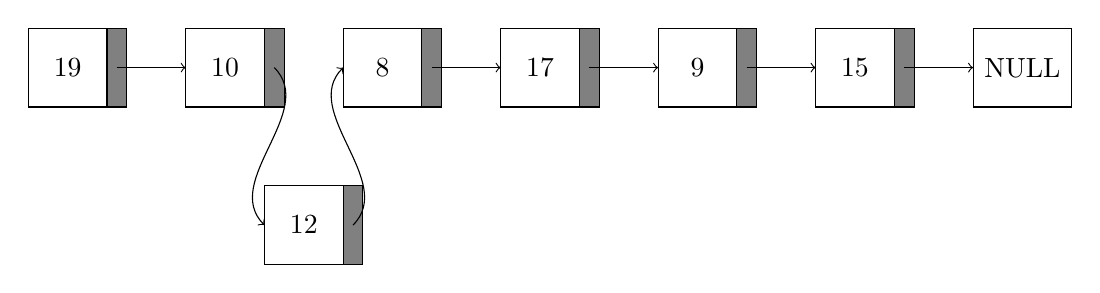
\begin{tikzpicture}
        % Draw the nodes of the linked list
        \draw (0, 0) rectangle (1, 1);
        \node at (0.5, 0.5) {19};
        \draw[fill=gray] (1, 1) rectangle (1.25, 0);

        \draw (2, 0) rectangle (3, 1);
        \node at (2.5, 0.5) {10};
        \draw[fill=gray] (3, 1) rectangle (3.25, 0);

        \draw (4, 0) rectangle (5, 1);
        \node at (4.5, 0.5) {8};
        \draw[fill=gray] (5, 1) rectangle (5.25, 0);

        \draw (6, 0) rectangle (7, 1);
        \node at (6.5, 0.5) {17};
        \draw[fill=gray] (7, 1) rectangle (7.25, 0);

        \draw (8, 0) rectangle (9, 1);
        \node at (8.5, 0.5) {9};
        \draw[fill=gray] (9, 1) rectangle (9.25, 0);

        \draw (10, 0) rectangle (11, 1);
        \node at (10.5, 0.5) {15};
        \draw[fill=gray] (11, 1) rectangle (11.25, 0);

        \draw (12, 0) rectangle (13.25, 1);
        \node at (12.625, 0.5) {NULL};

        % Insert the element 12 at index 2
        \draw (3, -1) rectangle (4, -2);
        \node at (3.5, -1.5) {12};
        \draw[fill=gray] (4, -1) rectangle (4.25, -2);

        % Draw the arrows between the nodes
        \draw[->] (1.125, 0.5) -- (2, 0.5);
        \draw[->] (5.125, 0.5) -- (6, 0.5);
        \draw[->] (7.125, 0.5) -- (8, 0.5);
        \draw[->] (9.125, 0.5) -- (10, 0.5);
        \draw[->] (11.125, 0.5) -- (12, 0.5);

        % Draw curved arrows for the inserted element
        \draw[->] (3.125, 0.5) to [out=315, in=135] (3.0, -1.5);
        \draw[->] (4.125, -1.5) to [out=45, in=225] (4.0, 0.5);
    \end{tikzpicture}
    \caption{Linked List Insertion}
    \label{fig:linked-list-insertion}
\end{figure}

Figure \ref{fig:linked-list-insertion} shows the visual representation of the
insertion operation in a linked list. The element 12 is inserted at index 2 of
the linked list, and the existing nodes are adjusted to accommodate the new
node. 

% Code example for linked list insertion
\begin{lstlisting}[language=C++, caption={Linked List Insertion}, label={lst:linked-list-insertion}]
struct Node {
    int data;
    Node *next;
    
    Node(int data) {
        this->data = data;
        this->next = NULL;
    }
};

int main() {
    Node *first = new Node(19);
    Node *second = new Node(10);
    Node *third = new Node(8);
    Node *fourth = new Node(17);
    Node *fifth = new Node(9);
    Node *sixth = new Node(15);

    Node *head = first;

    first->next = second;
    second->next = third;
    third->next = fourth;
    fourth->next = fifth;
    fifth->next = sixth;

    Node *newNode = new Node(12);
    Node *temp = head;
    int index = 2;

    for (int i = 0; i < index - 1; i++) {
        temp = temp->next;
    }

    newNode->next = temp->next;
    temp->next = newNode;

    return 0;
}
\end{lstlisting}

Code \ref{lst:linked-list-insertion} shows the code for inserting an element in
a linked list in C++. The code snippet defines a structure \texttt{Node} that
contains a data part and a next part that points to the next node in the
sequence. It then creates a linked list with nodes containing data values 19,
10, 8, 17, 9, and 15. The element 12 is inserted at index 2 of the linked list,
and the existing nodes are adjusted to accommodate the new node.

\subsubsection{Deletion}

The \textbf{\textit{deletion}} operation is used to remove a node from a linked
list at a specific position. The node at the specified position is removed, and
the existing nodes are adjusted to maintain the integrity of the list.

% TikZ diagram for linked list deletion
\begin{figure}[h]
    \centering
    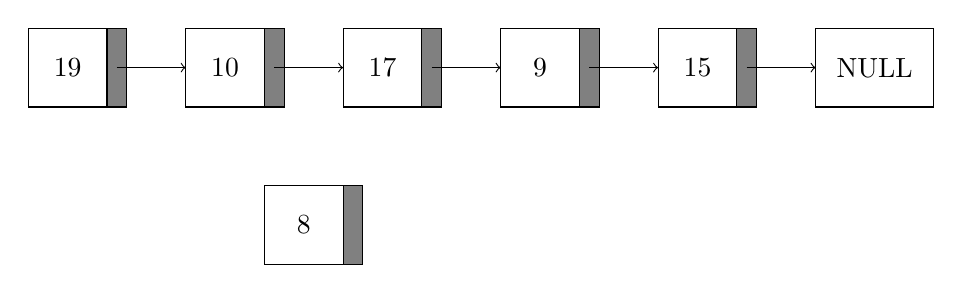
\begin{tikzpicture}
        % Draw the nodes of the linked list
        \draw (0, 0) rectangle (1, 1);
        \node at (0.5, 0.5) {19};
        \draw[fill=gray] (1, 1) rectangle (1.25, 0);

        \draw (2, 0) rectangle (3, 1);
        \node at (2.5, 0.5) {10};
        \draw[fill=gray] (3, 1) rectangle (3.25, 0);

        % \draw (4, 0) rectangle (5, 1);
        % \node at (4.5, 0.5) {8};
        % \draw[fill=gray] (5, 1) rectangle (5.25, 0);

        \draw (4, 0) rectangle (5, 1);
        \node at (4.5, 0.5) {17};
        \draw[fill=gray] (5, 1) rectangle (5.25, 0);

        \draw (6, 0) rectangle (7, 1);
        \node at (6.5, 0.5) {9};
        \draw[fill=gray] (7, 1) rectangle (7.25, 0);

        \draw (8, 0) rectangle (9, 1);
        \node at (8.5, 0.5) {15};
        \draw[fill=gray] (9, 1) rectangle (9.25, 0);

        \draw (10, 0) rectangle (11.5, 1);
        \node at (10.75, 0.5) {NULL};

        % Delete the element at index 2
        \draw (3, -1) rectangle (4, -2);
        \node at (3.5, -1.5) {8};
        \draw[fill=gray] (4, -1) rectangle (4.25, -2);

        % Draw the arrows between the nodes
        \draw[->] (1.125, 0.5) -- (2, 0.5);
        \draw[->] (3.125, 0.5) -- (4, 0.5);
        \draw[->] (5.125, 0.5) -- (6, 0.5);
        \draw[->] (7.125, 0.5) -- (8, 0.5);
        \draw[->] (9.125, 0.5) -- (10, 0.5); 
    \end{tikzpicture}
    \caption{Linked List Deletion}
    \label{fig:linked-list-deletion}
\end{figure}

Figure \ref{fig:linked-list-deletion} shows the visual representation of the
deletion operation in a linked list. The element 10 is deleted from index 2 of
the linked list, and the existing nodes are adjusted to maintain the integrity
of the list.

% Code example for linked list deletion
\begin{lstlisting}[language=C++, caption={Linked List Deletion}, label={lst:linked-list-deletion}]
struct Node {
    int data;
    Node *next;
    
    Node(int data) {
        this->data = data;
        this->next = NULL;
    }
};

int main() {
    Node *first = new Node(19);
    Node *second = new Node(10);
    Node *third = new Node(8);
    Node *fourth = new Node(17);
    Node *fifth = new Node(9);
    Node *sixth = new Node(15);

    Node *head = first;

    first->next = second;
    second->next = third;
    third->next = fourth;
    fourth->next = fifth;
    fifth->next = sixth;

    Node *temp = head;
    int index = 2;

    for (int i = 0; i < index - 1; i++) {
        temp = temp->next;
    }

    Node *deletedNode = temp->next;
    temp->next = temp->next->next;
    delete deletedNode;

    return 0;
}
\end{lstlisting}

Code \ref{lst:linked-list-deletion} shows the code for deleting an element from
a linked list in C++. The code snippet defines a structure \texttt{Node} that
contains a data part and a next part that points to the next node in the
sequence. It then creates a linked list with nodes containing data values 19,
10, 8, 17, 9, and 15. The element 10 is deleted from index 2 of the linked
list, and the existing nodes are adjusted to maintain the integrity of the list.

\subsubsection{Searching}

The \textbf{\textit{searching}} operation is used to find a specific element in
a linked list. The list is traversed from the head node to the last node to find
the element with the specified value.

% TikZ diagram for linked list searching
\begin{figure}[h]
    \centering
    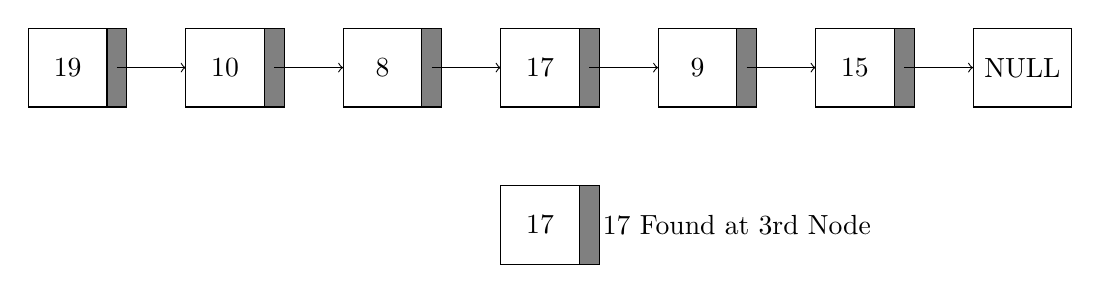
\begin{tikzpicture}
        % Draw the nodes of the linked list
        \draw (0, 0) rectangle (1, 1);
        \node at (0.5, 0.5) {19};
        \draw[fill=gray] (1, 1) rectangle (1.25, 0);

        \draw (2, 0) rectangle (3, 1);
        \node at (2.5, 0.5) {10};
        \draw[fill=gray] (3, 1) rectangle (3.25, 0);

        \draw (4, 0) rectangle (5, 1);
        \node at (4.5, 0.5) {8};
        \draw[fill=gray] (5, 1) rectangle (5.25, 0);

        \draw (6, 0) rectangle (7, 1);
        \node at (6.5, 0.5) {17};
        \draw[fill=gray] (7, 1) rectangle (7.25, 0);

        \draw (8, 0) rectangle (9, 1);
        \node at (8.5, 0.5) {9};
        \draw[fill=gray] (9, 1) rectangle (9.25, 0);

        \draw (10, 0) rectangle (11, 1);
        \node at (10.5, 0.5) {15};
        \draw[fill=gray] (11, 1) rectangle (11.25, 0);

        \draw (12, 0) rectangle (13.25, 1);
        \node at (12.625, 0.5) {NULL};

        % Search for the element 17
        \draw (6, -1) rectangle (7, -2);
        \node at (6.5, -1.5) {17};
        \draw[fill=gray] (7, -1) rectangle (7.25, -2);

        % Label the search result
        \node at (9, -1.5) {17 Found at 3rd Node};

        % Draw the arrows between the nodes
        \draw[->] (1.125, 0.5) -- (2, 0.5);
        \draw[->] (3.125, 0.5) -- (4, 0.5);
        \draw[->] (5.125, 0.5) -- (6, 0.5);
        \draw[->] (7.125, 0.5) -- (8, 0.5);
        \draw[->] (9.125, 0.5) -- (10, 0.5);
        \draw[->] (11.125, 0.5) -- (12, 0.5);
    \end{tikzpicture}
    \caption{Linked List Searching}
    \label{fig:linked-list-searching}
\end{figure}

Figure \ref{fig:linked-list-searching} shows the visual representation of the
searching operation in a linked list. The element 17 is searched for in the
linked list, and the list is traversed from the head node to the last node to
find the element with the specified value.

% Code example for linked list searching
\begin{lstlisting}[language=C++, caption={Linked List Searching}, label={lst:linked-list-searching}]
struct Node {
    int data;
    Node *next;
    
    Node(int data) {
        this->data = data;
        this->next = NULL;
    }
};

int main() {
    Node *first = new Node(19);
    Node *second = new Node(10);
    Node *third = new Node(8);
    Node *fourth = new Node(17);
    Node *fifth = new Node(9);
    Node *sixth = new Node(15);

    Node *head = first;

    first->next = second;
    second->next = third;
    third->next = fourth;
    fourth->next = fifth;
    fifth->next = sixth;

    int searchValue = 17;
    Node *temp = head;
    int position = 1;

    while (temp != NULL) {
        if (temp->data == searchValue) {
            break;
        }
        temp = temp->next;
        position++;
    }

    return 0;
}
\end{lstlisting}
    
Code \ref{lst:linked-list-searching} shows the code for searching an element in
a linked list in C++. The code snippet defines a structure \texttt{Node} that
contains a data part and a next part that points to the next node in the
sequence. It then creates a linked list with nodes containing data values 19,
10, 8, 17, 9, and 15. The element 17 is searched for in the linked list, and
the list is traversed from the head node to the last node to find the element
with the specified value.

% \subsection{Complexity Analysis of Linked Lists}

\section{Comparison of Arrays and Linked Lists}

Unlike arrays, linked lists do not have a fixed size and can grow dynamically
by adding new nodes. This makes linked lists more flexible and efficient for
insertion and deletion operations, as they do not require shifting elements to
accommodate new elements. However, linked lists have higher memory overhead due
to the additional pointers in each node.

Arrays are more efficient for random access operations, as elements can be
accessed directly using their index. In contrast, linked lists require
traversing the list from the head node to the desired node, which can be slower
for large lists. Arrays also have better cache locality, as elements are stored
contiguously in memory, leading to faster access times.

Thus, if the application requires frequent insertion and deletion operations
with a dynamic size, linked lists are a better choice. On the other hand, if the
application requires frequent random access operations and has a fixed size,
arrays are more suitable.

\section{Summary}

In this chapter, we discussed arrays and linked lists as fundamental data
structures in computer science. We covered the basic concepts, operations, and
implementations of arrays and linked lists, along with their comparison in terms
of performance and memory usage. We also explored different types of linked
lists, such as singly linked lists, doubly linked lists, circular linked lists,
and doubly circular linked lists, and discussed the operations on linked lists,
such as insertion, deletion, and searching. Finally, we compared arrays and
linked lists based on their characteristics and use cases.

\section{Coding Exercises}

\begin{enumerate}
    % Reverse an Array
    \item \textbf{Reverse an Array:} Write a C++ program to reverse an array of
    integers. The program should take the size of the array and the elements of
    the array as input and output the reversed array.
    \begin{enumerate}
        \item Declare an array of integers with a fixed size.
        \begin{align*}
            \text{int arr[6];}
        \end{align*}
        \item Initialize the array with the input elements.
        \begin{align*}
            \text{arr = \{19, 10, 8, 17, 9, 15\};}
        \end{align*}
        \item Reverse the array using a loop. \\
        \begin{center}
            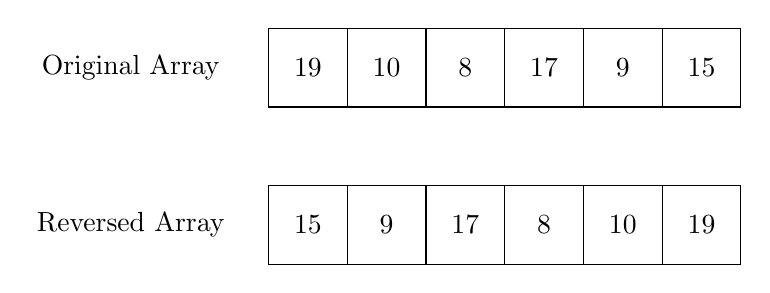
\begin{tikzpicture}[scale=1]
                \draw (0, 0) grid (6, 1);
                \node at (0.5, 0.5) {19};
                \node at (1.5, 0.5) {10};
                \node at (2.5, 0.5) {8};
                \node at (3.5, 0.5) {17};
                \node at (4.5, 0.5) {9};
                \node at (5.5, 0.5) {15};
                \node at (-1.75, 0.5) {Original Array};

                % \draw[->] (3, 0) -- (3, -1);

                \draw (0, -1) grid (6, -2);
                \node at (0.5, -1.5) {15};
                \node at (1.5, -1.5) {9};
                \node at (2.5, -1.5) {17};
                \node at (3.5, -1.5) {8};
                \node at (4.5, -1.5) {10};
                \node at (5.5, -1.5) {19};
                \node at (-1.75, -1.5) {Reversed Array};
            \end{tikzpicture}
        \end{center}
        \item Print the reversed array to the console.
        \begin{align*}
            \text{Reversed Array: 15, 9, 17, 8, 10, 19}
        \end{align*}
        \item Determine the \textbf{time complexity} and
        \textbf{space complexity} of the program.
    \end{enumerate}

    % Reverse a Linked List
    \item \textbf{Reverse a Linked List:} Write a C++ program to reverse a singly
    linked list. The program should take the elements of the linked list as input
    and output the reversed linked list.

    \begin{enumerate}
        \item Create a singly linked list with nodes containing the elements
        \begin{center}
            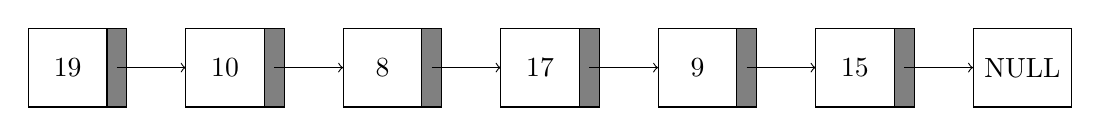
\begin{tikzpicture}
                \draw (0, 0) rectangle (1, 1);
                \node at (0.5, 0.5) {19};
                \draw[fill=gray] (1, 1) rectangle (1.25, 0);
    
                \draw (2, 0) rectangle (3, 1);
                \node at (2.5, 0.5) {10};
                \draw[fill=gray] (3, 1) rectangle (3.25, 0);
    
                \draw (4, 0) rectangle (5, 1);
                \node at (4.5, 0.5) {8};
                \draw[fill=gray] (5, 1) rectangle (5.25, 0);
    
                \draw (6, 0) rectangle (7, 1);
                \node at (6.5, 0.5) {17};
                \draw[fill=gray] (7, 1) rectangle (7.25, 0);
    
                \draw (8, 0) rectangle (9, 1);
                \node at (8.5, 0.5) {9};
                \draw[fill=gray] (9, 1) rectangle (9.25, 0);
    
                \draw (10, 0) rectangle (11, 1);
                \node at (10.5, 0.5) {15};
                \draw[fill=gray] (11, 1) rectangle (11.25, 0);
    
                \draw (12, 0) rectangle (13.25, 1);
                \node at (12.625, 0.5) {NULL};
    
                \draw[->] (1.125, 0.5) -- (2, 0.5);
                \draw[->] (3.125, 0.5) -- (4, 0.5);
                \draw[->] (5.125, 0.5) -- (6, 0.5);
                \draw[->] (7.125, 0.5) -- (8, 0.5);
                \draw[->] (9.125, 0.5) -- (10, 0.5);
                \draw[->] (11.125, 0.5) -- (12, 0.5);
            \end{tikzpicture}
        \end{center}
        \item Reverse the linked list using a loop.
        \begin{center}
            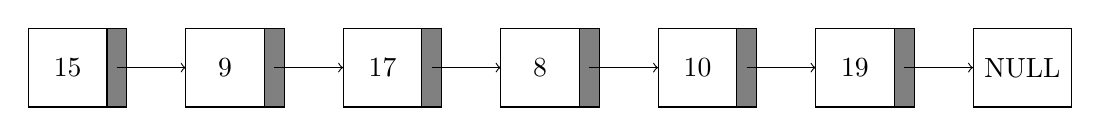
\begin{tikzpicture}
                \draw (0, 0) rectangle (1, 1);
                \node at (0.5, 0.5) {15};
                \draw[fill=gray] (1, 1) rectangle (1.25, 0);
    
                \draw (2, 0) rectangle (3, 1);
                \node at (2.5, 0.5) {9};
                \draw[fill=gray] (3, 1) rectangle (3.25, 0);
    
                \draw (4, 0) rectangle (5, 1);
                \node at (4.5, 0.5) {17};
                \draw[fill=gray] (5, 1) rectangle (5.25, 0);
    
                \draw (6, 0) rectangle (7, 1);
                \node at (6.5, 0.5) {8};
                \draw[fill=gray] (7, 1) rectangle (7.25, 0);
    
                \draw (8, 0) rectangle (9, 1);
                \node at (8.5, 0.5) {10};
                \draw[fill=gray] (9, 1) rectangle (9.25, 0);
    
                \draw (10, 0) rectangle (11, 1);
                \node at (10.5, 0.5) {19};
                \draw[fill=gray] (11, 1) rectangle (11.25, 0);
    
                \draw (12, 0) rectangle (13.25, 1);
                \node at (12.625, 0.5) {NULL};
    
                \draw[->] (1.125, 0.5) -- (2, 0.5);
                \draw[->] (3.125, 0.5) -- (4, 0.5);
                \draw[->] (5.125, 0.5) -- (6, 0.5);
                \draw[->] (7.125, 0.5) -- (8, 0.5);
                \draw[->] (9.125, 0.5) -- (10, 0.5);
                \draw[->] (11.125, 0.5) -- (12, 0.5);
            \end{tikzpicture}
        \end{center}
        \item Print the reversed linked list to the console.
        \begin{align*}
            \text{Reversed Linked List: 15, 9, 17, 8, 10, 19}
        \end{align*}
        \item Determine the \textbf{time complexity} and
        \textbf{space complexity} of the program.
    \end{enumerate}
    
    % Search a Circular Linked List
    \item \textbf{Search a Circular Linked List:} Write a C++ program to search
    for an element in a circular linked list. The program should take the elements
    of the circular linked list as input and output the position of the element
    in the list. If the current node's next pointer points to the head node, the
    list is circular. If the element is not found in the list, output "Element not
    found." Else, output the position of the element in the list.
    \begin{enumerate}
        \item Create a circular linked list with nodes containing the elements \\
        \begin{center}
            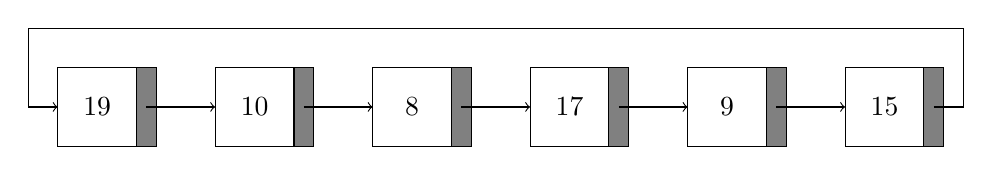
\begin{tikzpicture}[scale=1]
                % Draw the nodes of the circular linked list
                \draw (0, 0) rectangle (1, 1);
                \node at (0.5, 0.5) {19};
                \draw[fill=gray] (1, 1) rectangle (1.25, 0);
        
                \draw (2, 0) rectangle (3, 1);
                \node at (2.5, 0.5) {10};
                \draw[fill=gray] (3, 1) rectangle (3.25, 0);
        
                \draw (4, 0) rectangle (5, 1);
                \node at (4.5, 0.5) {8};
                \draw[fill=gray] (5, 1) rectangle (5.25, 0);
        
                \draw (6, 0) rectangle (7, 1);
                \node at (6.5, 0.5) {17};
                \draw[fill=gray] (7, 1) rectangle (7.25, 0);
        
                \draw (8, 0) rectangle (9, 1);
                \node at (8.5, 0.5) {9};
                \draw[fill=gray] (9, 1) rectangle (9.25, 0);
        
                \draw (10, 0) rectangle (11, 1);
                \node at (10.5, 0.5) {15};
                \draw[fill=gray] (11, 1) rectangle (11.25, 0);
        
                % Draw the arrows between the nodes
                \draw[->] (1.125, 0.5) -- (2, 0.5);
                \draw[->] (3.125, 0.5) -- (4, 0.5);
                \draw[->] (5.125, 0.5) -- (6, 0.5);
                \draw[->] (7.125, 0.5) -- (8, 0.5);
                \draw[->] (9.125, 0.5) -- (10, 0.5);
        
                % Add Curved Arrow from last node to first node
                % \draw[->] (11.125, 0.5) to [out=45, in=135] (0, 0.5);
                \draw[->] (11.125, 0.5)
                    -- (11.5, 0.5)
                    -- (11.5, 1.5)
                    -- (-0.375, 1.5)
                    -- (-0.375, 0.5)
                    -- (0, 0.5);
            \end{tikzpicture}
        \end{center}
        \item Using \textit{cin}, take the input element to search for
        \begin{align*}
            \text{Search Element: 21}
        \end{align*}
        \item Search for the element in the circular linked list
        \begin{align*}
            \text{Output: Element not found.}
        \end{align*}
        \item Determine the \textbf{time complexity} and
        \textbf{space complexity} of the program.
    \end{enumerate}
\end{enumerate}

 %%%%%%%%%%%%%%%%%%%%%%%%%%%%%%%%%%%%
%%%%%~ NEW CHAPTER STARTS HERE %%%%%
%%%%%%%%%%%%%%%%%%%%%%%%%%%%%%%%%%%%
\chapter{Stacks and Queues}

\section{Introduction}

\section{Stacks}

\subsection{Operations on Stacks}

\subsubsection{Push}

\subsubsection{Pop}

\subsubsection{Peek}

\subsubsection{isEmpty}

\subsubsection{isFull}

\subsection{Complexity Analysis of Stacks}

\subsection{Implementation of Stacks Using Arrays}

\subsection{Implementation of Stacks Using Linked Lists}

\section{Queues}

\subsection{Types of Queues}

\subsubsection{Linear Queue}

\subsubsection{Circular Queue}

\subsubsection{Priority Queue}

\subsubsection{Double-ended Queue (Deque)}

\subsection{Operations on Queues}

\subsubsection{Enqueue}

\subsubsection{Dequeue}

\subsubsection{Front}

\subsubsection{Rear}

\subsection{Complexity Analysis of Queues}

\subsection{Implementation of Queues Using Arrays}

\subsection{Implementation of Queues Using Linked Lists}

\section{Comparison of Stacks and Queues}

\section{Summary}

%%%%%%%%%%%%%%%%%%%%%%%%%%%%%%%%%%%%
%%%%%~ NEW CHAPTER STARTS HERE %%%%%
%%%%%%%%%%%%%%%%%%%%%%%%%%%%%%%%%%%%
\chapter{Trees}

\section{Introduction}

\section{Properties of Trees}

\subsection{Root Node}

\subsection{Parent Node}

\subsection{Child Node}

\subsection{Leaf Node}

\subsection{Ancestors}

\subsection{Siblings}

\subsection{Descendants}

\subsection{Height of a Tree}

\subsection{Depth of a Node}

\subsection{Degree of a Node}

\subsection{Level of a Node}

\subsection{Subtree}

\section{Types of Trees}

\subsection{Binary Tree}

\subsubsection{Types of Binary Trees}

\paragraph{Left-skewed Binary Tree}

\paragraph{Right-skewed Binary Tree}

\paragraph{Complete Binary Tree}

\subsection{Ternary Tree}

\subsection{N-ary Tree}

\subsection{Binary Search Tree}

\subsection{AVL Tree}

\subsection{Red-Black Tree}

\section{Basic Operations on Trees}

\subsection{Creation of a Tree}

\subsection{Insertion}

\subsection{Deletion}

\subsection{Searching}

\subsection{Traversal}

\subsubsection{Preorder Traversal}

\subsubsection{Inorder Traversal}

\subsubsection{Postorder Traversal}

\subsubsection{Level-order Traversal}

\section{Complexity Analysis of Trees}

\section{Summary}

%%%%%%%%%%%%%%%%%%%%%%%%%%%%%%%%%%%%
%%%%%~ NEW CHAPTER STARTS HERE %%%%%
%%%%%%%%%%%%%%%%%%%%%%%%%%%%%%%%%%%%
\chapter{Graphs}

\section{Introduction}

\section{Properties of Graphs}

\subsection{Vertex}

\subsection{Edge}

\subsection{Degree of a Vertex}

\subsection{Path}

\section{Types of Graphs}

\subsection{Finite Graph}

\subsection{Infinite Graph}

\subsection{Trivial Graph}

\subsection{Simple Graph}

\subsection{Multi Graph}

\subsection{Null Graph}

\subsection{Complete Graph}

\subsection{Pseudo Graph}

\subsection{Regular Graph}

\subsection{Bipartite Graph}

\subsection{Labelled Graph}

\subsection{Weighted Graph}

\subsection{Directed Graph}

\subsection{Undirected Graph}

\subsection{Connected Graph}

\subsection{Disconnected Graph}

\subsection{Cyclic Graph}

\subsection{Acyclic Graph}

\subsection{Directed Acyclic Graph (DAG)}

\subsection{Digraph}

\subsection{Subgraph}

\section{Operations on Graphs}

\subsection{Creation of a Graph}

\subsection{Insertion}

\subsubsection{Insertion of a Vertex}

\subsubsection{Insertion of an Edge}

\subsection{Deletion}

\subsubsection{Deletion of a Vertex}

\subsubsection{Deletion of an Edge}

\subsection{Traversal}

\subsubsection{Depth First Search (DFS)}

\subsubsection{Breadth First Search (BFS)}

\subsection{Shortest Path}

\subsection{Minimum Spanning Tree}

\section{Complexity Analysis of Graphs}

\section{Summary}

%%%%%%%%%%%%%%%%%%%%%%%%%%%%%%%%%%%%
%%%%%~ NEW CHAPTER STARTS HERE %%%%%
%%%%%%%%%%%%%%%%%%%%%%%%%%%%%%%%%%%%
\chapter{Sorting and Searching}

\section{Introduction}

\section{Sorting}

\subsection{Types of Sorting Algorithms}

\subsubsection{Bubble Sort}

\subsubsection{Selection Sort}

\subsubsection{Insertion Sort}

\subsubsection{Merge Sort}

\subsubsection{Quick Sort}

\subsubsection{Heap Sort}

\subsubsection{Radix Sort}

\subsubsection{Counting Sort}

\subsubsection{Bucket Sort}

\subsection{Comparison of Sorting Algorithms}

\section{Searching}

\subsection{Types of Searching Algorithms}

\subsubsection{Linear Search}

\subsubsection{Binary Search}

\subsubsection{Jump Search}

\subsubsection{Interpolation Search}

\subsubsection{Exponential Search}

\subsubsection{Fibonacci Search}

\subsubsection{Ternary Search}

\subsection{Comparison of Searching Algorithms}

\section{Summary}

%%%%%%%%%%%%%%%%%%%%%%%%%%%%%%%%%%%%
%%%%%~ NEW CHAPTER STARTS HERE %%%%%
%%%%%%%%%%%%%%%%%%%%%%%%%%%%%%%%%%%%
\chapter{Hashing}

\section{Introduction}

\section{Hash Table}

\section{Hash Function}

\section{Collision Resolution Techniques}

\subsection{Separate Chaining}

\subsection{Open Addressing}

\subsubsection{Linear Probing}

\subsubsection{Quadratic Probing}

\subsubsection{Double Hashing}

\section{Complexity Analysis of Hashing}

\section{Summary}

%%%%%%%%%%%%%%%%%%%%%%%%%%%%%%%%%%%%
%%%%%~ NEW CHAPTER STARTS HERE %%%%%
%%%%%%%%%%%%%%%%%%%%%%%%%%%%%%%%%%%%
\chapter{Advanced Data Structures and Algorithms}

\section{Introduction}

\section{Advanced Data Structures}

\subsection{Segment Tree}

\subsection{Fenwick Tree}

\subsection{Suffix Tree}

\subsection{Suffix Array}

\subsection{Trie}

\subsection{Heap}

\subsection{Disjoint Set}

\subsection{Skip List}

\subsection{Splay Tree}

\subsection{Bloom Filter}

\subsection{KD Tree}

\subsection{Quad Tree}

\subsection{Octree}

\subsection{B-Tree}

\subsection{B+ Tree}

\subsection{R-Tree}

\subsection{X-Tree}

\subsection{Y-Tree}

\subsection{Z-Tree}

\section{Advanced Algorithms}

\subsection{Dynamic Programming}

\subsection{Greedy Algorithms}

\subsection{Backtracking}

\subsection{Divide and Conquer}

\subsection{Branch and Bound}

\subsection{Randomized Algorithms}

\subsection{Approximation Algorithms}

\subsection{String Matching Algorithms}

\subsection{Pattern Searching Algorithms}

\subsection{Cryptography Algorithms}

\subsection{Geometric Algorithms}

\subsection{Graph Algorithms}

\subsection{Network Flow Algorithms}

\subsection{Game Theory Algorithms}

\subsection{Quantum Algorithms}

\section{Summary}

%%%%%%%%%%%%%%%%%%%%%%%%%%%%%%%%%%%%
%%%%%~ NEW CHAPTER STARTS HERE %%%%%
%%%%%%%%%%%%%%%%%%%%%%%%%%%%%%%%%%%%
\chapter{Applications of Data Structures and Algorithms}

\section{Applications in Computer Science}

\subsection{Operating Systems}

\subsection{Database Management Systems}

\subsection{Compiler Design}

\subsection{Networking}

\subsection{Artificial Intelligence}

\subsection{Machine Learning}

\subsection{Computer Graphics}

\subsection{Computer Vision}

\subsection{Robotics}

\subsection{Web Development}

\subsection{Mobile Development}

\subsection{Game Development}

\subsection{Cybersecurity}

\subsection{Quantum Computing}

\section{Applications in Real Life}

\subsection{Social Media}

\subsection{E-commerce}

\subsection{Healthcare}

\subsection{Finance}

\subsection{Transportation}

\subsection{Education}

\subsection{Agriculture}

\subsection{Manufacturing}

\subsection{Entertainment}

\subsection{Sports}

\subsection{Travel}

\subsection{Telecommunications}

\subsection{Energy}

\subsection{Environment}

\subsection{Politics}

\subsection{Military}

\section{Summary}

\chapter{References}

\begin{enumerate}[label={\textbf{\Alph*.}}]
  \item \textbf{Books}
    \begin{itemize}
      \item Vishwas R. (2023). Data Structure Handbook. Dr. Vishwas Raval. ISBN: 978-9359063591
      \item Cormen, T. H., Leiserson, C. E., Rivest, R. L., \& Stein, C. (2022). Introduction to algorithms. MIT press. ISBN: 978-0262046305
      \item Erickson, J. (2019). Algorithms. ISBN: 978-1792644832
    \end{itemize}
  \item \textbf{Other Sources}
    \begin{itemize}
      \item Tutorialspoint. (n.d.). Data Structures Basics. Data Structure Basics. \url{https://www.tutorialspoint.com/data_structures_algorithms/data_structures_basics.htm}
      \item Algorithm Archive · Arcane Algorithm Archive. (n.d.). \url{https://www.algorithm-archive.org/}
    \end{itemize}
\end{enumerate}

\end{document}
